\documentclass[aspectratio=169]{beamer}

% Setup
% Thesis Team Setup - Custom Setup for Candidate, Supervisor, Co-Supervisors in Beamer
% Place this file in your project directory and \input{thesis_team_setup.tex} in your main .tex

% Required packages
\usepackage{tabularx}
\usepackage[british]{babel}
\usepackage[utf8]{inputenc}
\usepackage{graphicx,hyperref,ru,url}
\usepackage{lmodern,tabularx,background,tikz}
\usepackage{scrextend}
\usepackage[skip=2pt]{caption}
\usepackage{subcaption}
\usepackage{xcolor}
\usepackage{fontawesome5}
\usepackage{tcolorbox}
\usepackage{tikz}
\usepackage{mdwlist}

% Bibliography setup for [Author, et al., Year] format
\usepackage[style=authoryear,backend=biber,maxcitenames=1,mincitenames=1]{biblatex}
\addbibresource{references.bib}
\usetikzlibrary{positioning,arrows.meta,calc,automata,decorations.pathreplacing}
\tikzset{
  accepting/.style={circle, draw, double, minimum size=7mm}
}

% Team member macros (LaTeX2e, needs \makeatletter...\makeatother)
\makeatletter
\newcommand{\candidate}[1]{\def\@candidate{#1}}
\newcommand{\supervisor}[1]{\def\@supervisor{#1}}
\newcommand{\cosupervisors}[1]{\def\@cosupervisors{#1}}
\newcommand{\printthesisteam}{
  \vspace{0.3cm}
  \begin{center}
    \begin{tabular}{@{}p{0.28\linewidth}@{\hspace{0.05\linewidth}}p{0.28\linewidth}@{\hspace{0.05\linewidth}}p{0.35\linewidth}@{}}
      \raggedright\footnotesize \textbf{Candidate}: \@candidate &
      \centering\footnotesize \textbf{Supervisor}: \@supervisor &
      \raggedleft\footnotesize \textbf{Co-Supervisor}: \@cosupervisors \\
    \end{tabular}
  \end{center}
}
\makeatother

% Title and metadata
\title[RU style for Beamer]{A New Compression Technique for Repetitive Tries}
\author[Davide Tonetto]{\changefontsizes{12pt} \textsc{Davide Tonetto}}
\institute[Ca' Foscari]{
\changefontsizes{10pt}
  \textsc{Ca’ Foscari University of Venice \\
Department of Environmental Sciences, Informatics and Statistics}
}
\date[master thesis]{
{\changefontsizes{14pt}
  \textsc{Master's Thesis Defense} \\[0.3cm] \changefontsizes{8pt}
  Computer Science and Information Technology\\[-0.5em] \textit{Artificial Intelligence and Data Engineering} }\\[0.5cm]
  \textsc{6th November 2025}
  \printthesisteam
}

% Watermark background (logo on right, faint, scaled, shifted)
\setbeamertemplate{background}{
  \begin{tikzpicture}[remember picture,overlay]
    \node[anchor=east, opacity=0.05, scale=0.9, yshift=-0.72cm] at ([xshift=3.3cm]current page.east) 
      {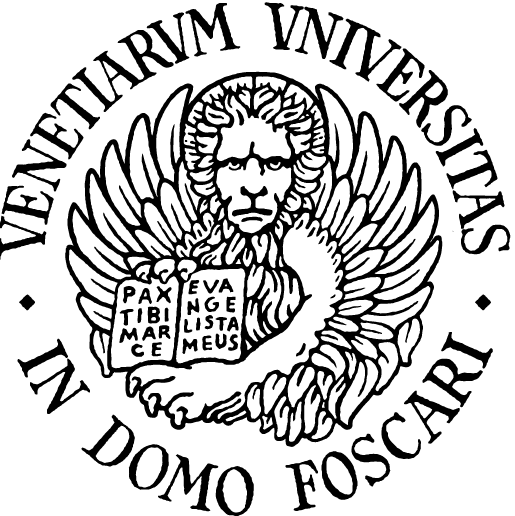
\includegraphics[height=0.8\paperheight]{UNIVE_square_black.png}};
  \end{tikzpicture}
}

\newcommand{\fancysectionframe}[2][]{%
  \begin{frame}[plain]
    \centering
    \vfill
    {\color{rured} \bfseries \LARGE #2}
    \ifx&#1&\else
      \\[0.5em]
      {\color{black} \large #1}
    \fi
    \par\vspace{0.5ex}
    {\color{rured}\rule{0.45\paperwidth}{1.7pt}}
    \vfill
  \end{frame}
}

% Palette di colori ad alta visibilità e colorblind-safe (Okabe–Ito)
\definecolor{oiBlue}{HTML}{0072B2}
\definecolor{oiSkyBlue}{HTML}{56B4E9}
\definecolor{oiOrange}{HTML}{E69F00}
\definecolor{oiGreen}{HTML}{009E73}
\definecolor{oiVermillion}{HTML}{D55E00}
\definecolor{oiPurple}{HTML}{CC79A7}
\definecolor{oiLightGrey}{HTML}{D3D3D3}
\definecolor{oiRed}{HTML}{FF0000}



\setbeamertemplate{caption}[numbered]

% Setup thesis team members
\candidate{Davide Tonetto}
\supervisor{Nicola Prezza}
\cosupervisors{Alessio Campanelli}



\begin{document}

\begin{frame}[plain]
	\titlepage
\end{frame}

% \begin{frame}
%   \frametitle{Outline}
%   \tableofcontents
% \end{frame}

\fancysectionframe{Introduction and Motivation}

\section{Introduction and Motivation}

\begin{frame}{Basic Definitions: Tries and Queries}
	\begin{columns}[c]
		\column{0.55\textwidth}
		% \textcolor{oiVermillion}{\textbf{Example Trie}}
		\begin{figure}
			\centering
			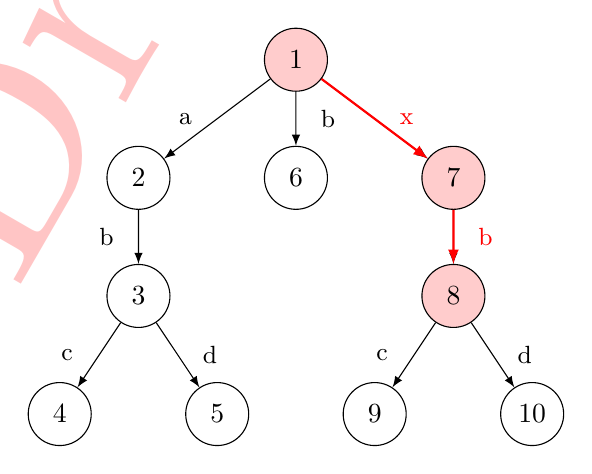
\begin{tikzpicture}[
					every node/.style={draw, circle, minimum size=8mm, inner sep=0pt},
					edge from parent/.style={draw, -latex},
					scale=1,
					level distance=1.5cm,
					sibling distance=2cm, % wider
					accepting/.style={double, fill=green!20},
					edge label/.style={font=\small, draw=none}
				]
				% Tree structure with named nodes
				\node[fill=red!20] (root) {1}
				child { node (a) {2}
				child { node (ab) {3}
				child { node[] (abc) {4} [label=below:{\texttt{abc}}] }
				child { node[] (abd) {5} [label=below:{\texttt{abd}}] }
				}
				}
				child {
						node[] (b) {6}
					}
				child { node[fill=red!20] (x) {7}
				child { node[fill=red!20] (xb) {8}
				child { node[] (xbc) {9} [label=below:{\texttt{xbc}}] }
				child { node[] (xbd) {10} [label=below:{\texttt{xbd}}] }
				}
				};

				% Edge coloring for the red path
				\draw[-latex, red, thick] (root) -- (x);
				\draw[-latex, red, thick] (x) -- (xb);

				% Edge labels using \path
				\path (root) -- (a) node[midway, left, edge label] {a};
				\path (root) -- (b) node[midway, right, edge label] {b};
				\path (a) -- (ab) node[midway, left, edge label] {b};
				\path (ab) -- (abc) node[midway, left, edge label] {c};
				\path (ab) -- (abd) node[midway, right, edge label] {d};

				\path (root) -- (x) node[midway, right, edge label, red] {x};
				\path (x) -- (xb) node[midway, right, edge label, red] {b};
				\path (xb) -- (xbc) node[midway, left, edge label] {c};
				\path (xb) -- (xbd) node[midway, right, edge label] {d};
			\end{tikzpicture}
			\caption{The language is $\{abc, abd, b, xbc, xbd\}$. The path for \texttt{xbd} is highlighted in red.}
			\label{fig:trie_example}
		\end{figure}
		\column{0.45\textwidth}
		\begin{block}{Trie}
			A trie is a \textcolor{oiVermillion}{\textbf{tree data structure}} optimized for \textcolor{oiRed}{\textbf{storing strings}} and performing \textcolor{oiPurple}{\textbf{fast prefix-based queries}}.
		\end{block}
		\textcolor{oiBlue}{\textbf{Prefix-Query for `xb'}} \\
		\small
		\begin{enumerate}
			\item Start at the root.
			\item Follow the edge labeled \texttt{x}.
			\item From there, follow the edge labeled \texttt{b}.
			\item There are two strings with prefix \texttt{xb}: \texttt{xbc} and \texttt{xbd}.
		\end{enumerate}
	\end{columns}
\end{frame}

\begin{frame}{Basic Definitions: Sub-Path Queries}
	\begin{columns}[c]
		\column{0.55\textwidth}
		\begin{figure}
			\centering
			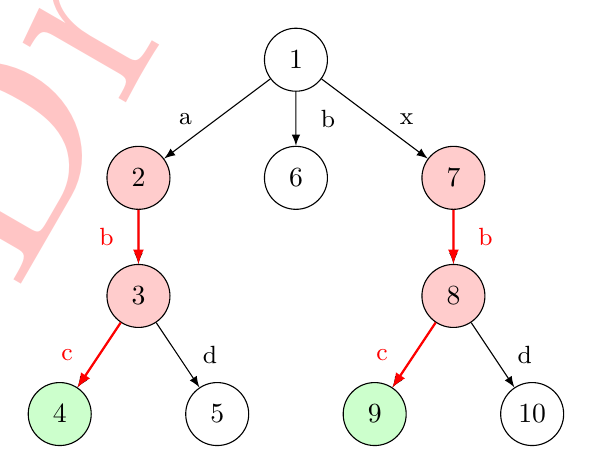
\begin{tikzpicture}[
					every node/.style={draw, circle, minimum size=8mm, inner sep=0pt},
					edge from parent/.style={draw, -latex},
					scale=1,
					level distance=1.5cm,
					sibling distance=2cm, % wider
					accepting/.style={double, fill=green!20},
					edge label/.style={font=\small, draw=none}
				]
				% Tree structure with named nodes
				\node[] (root) {1}
				child { node[fill=red!20] (a) {2}
				child { node[fill=red!20] (ab) {3}
				child { node[fill=green!20] (abc) {4} [label=below:{\texttt{abc}}] }
				child { node[] (abd) {5} [label=below:{\texttt{abd}}] }
				}
				}
				child {
						node[] (b) {6}
					}
				child { node[fill=red!20] (x) {7}
				child { node[fill=red!20] (xb) {8}
				child { node[fill=green!20] (xbc) {9} [label=below:{\texttt{xbc}}] }
				child { node[, ] (xbd) {10} [label=below:{\texttt{xbd}}] }
				}
				};

				% Edge coloring for the red path
				\draw[-latex, red, thick] (a) -- (ab);
				\draw[-latex, red, thick] (ab) -- (abc);
				\draw[-latex, red, thick] (x) -- (xb);
				\draw[-latex, red, thick] (xb) -- (xbc);

				% Edge labels using \path
				\path (root) -- (a) node[midway, left, edge label] {a};
				\path (root) -- (b) node[midway, right, edge label] {b};
				\path (a) -- (ab) node[midway, left, edge label, red] {b};
				\path (ab) -- (abc) node[midway, left, edge label, red] {c};
				\path (ab) -- (abd) node[midway, right, edge label] {d};

				\path (root) -- (x) node[midway, right, edge label] {x};
				\path (x) -- (xb) node[midway, right, edge label, red] {b};
				\path (xb) -- (xbc) node[midway, left, edge label, red] {c};
				\path (xb) -- (xbd) node[midway, right, edge label] {d};
			\end{tikzpicture}
			\caption{The language is $\{abc, abd, b, xbc, xbd\}$. The path for \texttt{xbd} is highlighted in red.}
			\label{fig:trie_example}
		\end{figure}

		\column{0.45\textwidth}
		\textcolor{oiBlue}{\textbf{Sub-Path Query}}
		\begin{itemize}
			\item \textbf{Definition:} Find label sequences starting from \textit{any} node
			\item \textbf{Advantage:} More flexible than prefix queries
		\end{itemize}
		\vspace{0.5cm}
		\textcolor{oiBlue}{\textbf{Example for `bc'}}
		\begin{itemize}
			\item Return the set of states reached by a path with label \texttt{bc}.
			\item In Figure \autoref{fig:trie_example}, states \texttt{4} and \texttt{9} are returned.
		\end{itemize}
	\end{columns}
\end{frame}

\begin{frame}{Motivations}
	\begin{columns}[t]
		\column{0.5\textwidth}
		\textcolor{oiVermillion}{\textbf{Why Tries Matter}}
		\begin{itemize}
			\item \textbf{Purpose:} Fundamental data structures for large string sets
			\item \textbf{Strength:} Efficient prefix-based queries
			\item \textbf{Challenge:} Memory consumption can be massive
		\end{itemize}

		\column{0.5\textwidth}
		\onslide<2->
		\textcolor{oiBlue}{\textbf{Real-World Applications}}
		\begin{itemize}
			\item \textbf{Text Processing:} Spell checking systems
			\item \textbf{Bioinformatics:} DNA/protein pattern matching
			\item \textbf{Databases:} String indexing and retrieval
		\end{itemize}
	\end{columns}
\end{frame}

\begin{frame}{Tries, DFAs and Minimization}
	\small
	\begin{itemize}
		\item<1-> \textcolor{oiBlue}{\textbf{Theoretical Foundation:}} A trie can be viewed as an \textbf{acyclic DFA}
		\item<2-> \textcolor{oiGreen}{\textbf{Minimization Principle:}} DFA minimization merges \textbf{Myhill--Nerode equivalent states}
		\item<3-> \textcolor{oiPurple}{\textbf{Algorithmic Solution:}} \textbf{Linear minimization} for acyclic DFAs~[\cite{revuz1992minimisation}]
	\end{itemize}
	\centering
	
	\begin{figure}
		\centering
		\scalebox{0.9}{%
			\begin{minipage}{\textwidth}
				\centering
				\onslide<4->
				\begin{subfigure}[b]{0.42\textwidth}
					\centering
					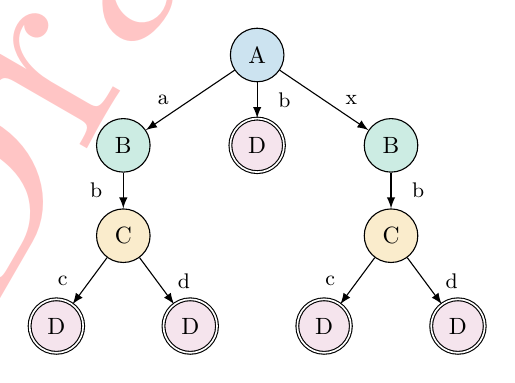
\begin{tikzpicture}[
							scale=0.85, transform shape,
							every node/.style={draw, circle, minimum size=8mm, inner sep=0pt},
							edge from parent/.style={draw, -latex},
							level distance=1.35cm,
							sibling distance=2cm, % wider
							accepting/.style={double},
							edge label/.style={font=\small, draw=none}
						]
						% Tree structure with named nodes
						\node[fill=oiBlue!20] (root) {A}
						child { node[fill=oiGreen!20] (a) {B}
						child { node[fill=oiOrange!20] (ab) {C}
						child { node[fill=oiPurple!20, accepting] (abc) {D} [label=below:{\texttt{abc}}] }
						child { node[fill=oiPurple!20, accepting] (abd) {D} [label=below:{\texttt{abd}}] }
						}
						}
						child{ node[fill=oiPurple!20, accepting] (b) {D} }
						child { node[fill=oiGreen!20] (x) {B}
						child { node[fill=oiOrange!20] (xb) {C}
						child { node[fill=oiPurple!20, accepting] (xbc) {D} [label=below:{\texttt{xbc}}] }
						child { node[fill=oiPurple!20, accepting] (xbd) {D} [label=below:{\texttt{xbd}}] }
						}
						};

						% Edge labels using \path
						\path (root) -- (a) node[midway, left, edge label] {a};
						\path (root) -- (b) node[midway, right, edge label] {b};
						\path (a) -- (ab) node[midway, left, edge label] {b};
						\path (ab) -- (abc) node[midway, left, edge label] {c};
						\path (ab) -- (abd) node[midway, right, edge label] {d};

						\path (root) -- (x) node[midway, right, edge label] {x};
						\path (x) -- (xb) node[midway, right, edge label] {b};
						\path (xb) -- (xbc) node[midway, left, edge label] {c};
						\path (xb) -- (xbd) node[midway, right, edge label] {d};
					\end{tikzpicture}
					\caption{Trie of \ref{fig:trie_example} with equivalence classes.}
					\label{fig:trie_for_minimization}
				\end{subfigure}
				\hfill
				\onslide<5->
				\begin{subfigure}[b]{0.42\textwidth}
					\centering
					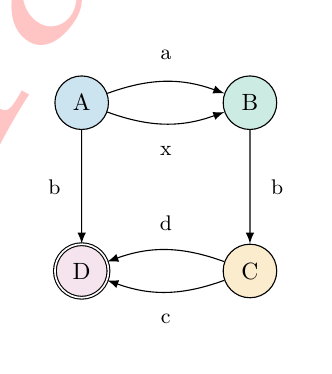
\begin{tikzpicture}[
							scale=0.85, transform shape,
							every node/.style={draw, circle, minimum size=8mm, inner sep=0pt},
							node distance=1.7cm,
							accepting/.style={double, fill=green!20},
							edge label/.style={font=\small, draw=none, midway}
						]
						\node[fill=oiBlue!20] (A) {A};
						\node[right=of A, fill=oiGreen!20] (B) {B};
						\node[below=of B, fill=oiOrange!20] (C) {C};
						\node[accepting, left=of C, fill=oiPurple!20] (D) {D};

						\path[-latex] (A) edge[bend left=20] node[above, edge label] {a} (B);
						\path[-latex] (A) edge[bend right=20] node[below, edge label] {x} (B);
						\path[-latex] (A) edge node[left, edge label] {b} (D);
						\path[-latex] (B) edge node[right, edge label] {b} (C);
						\path[-latex] (C) edge[bend left=20] node[below, edge label] {c} (D);
						\path[-latex] (C) edge[bend right=20] node[above, edge label] {d} (D);
					\end{tikzpicture}
					\caption{The minimized automaton.}
					\label{fig:minimized_automaton}
				\end{subfigure}
				\caption{An example of automaton minimization for trie of \ref{fig:trie_example}.}
				\label{fig:minimization_ex}
			\end{minipage}
		}%
	\end{figure}
\end{frame}

\begin{frame}{Challenges}
	\begin{columns}[c]
		\column{0.6\textwidth}
		\centering
		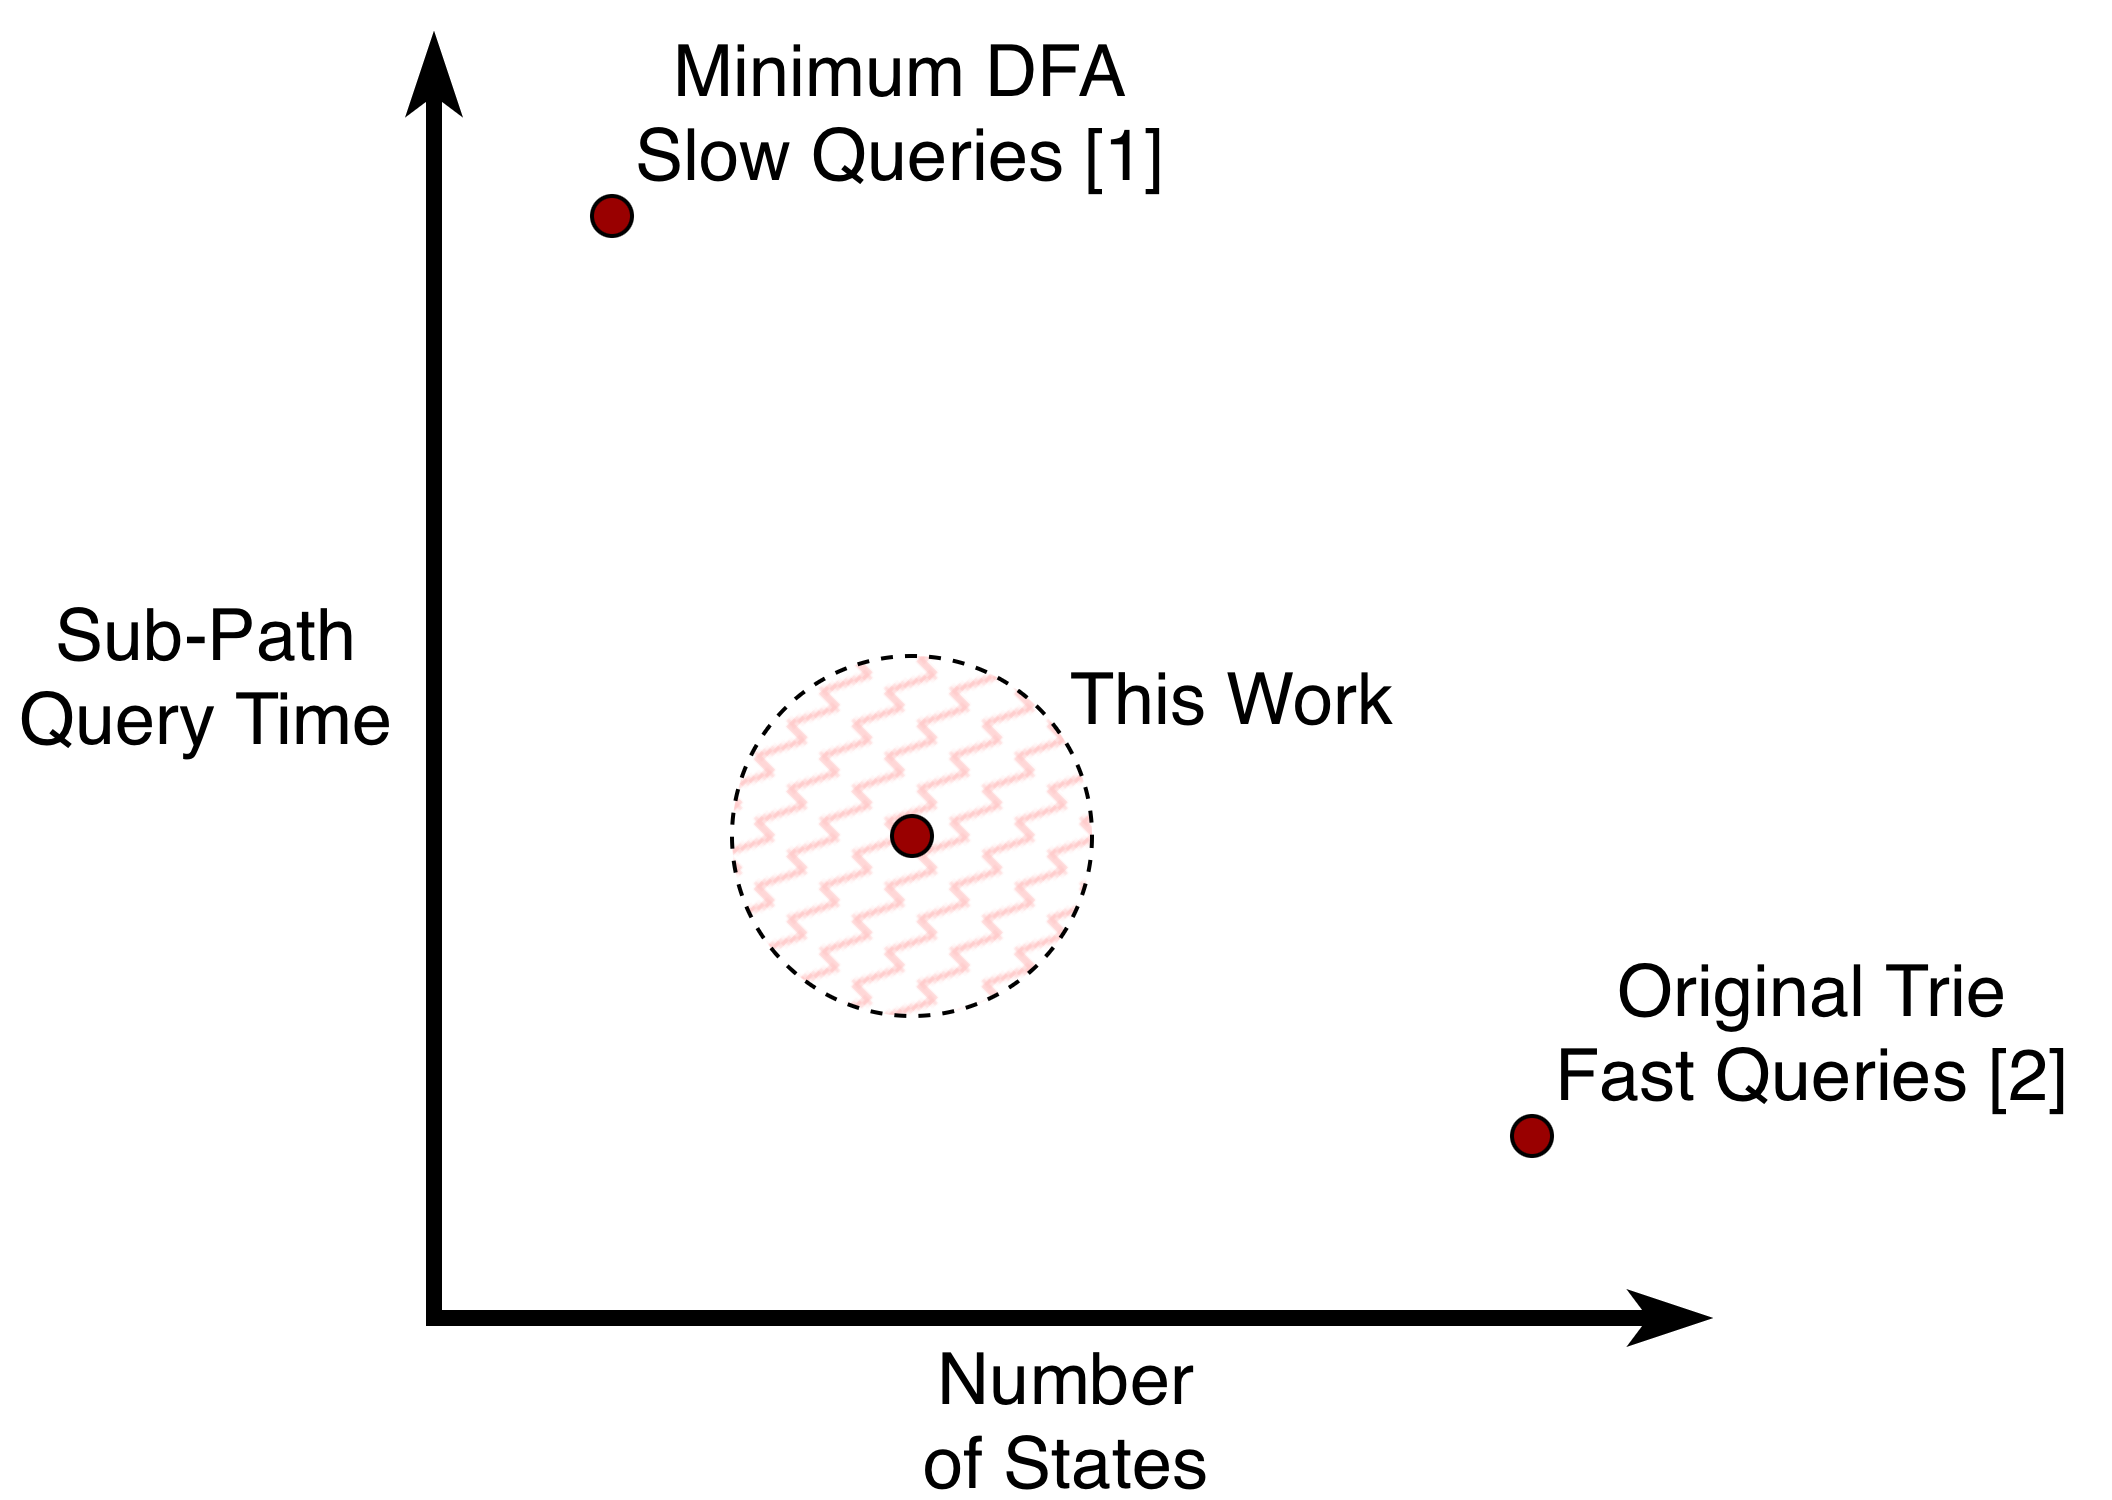
\includegraphics[width=\textwidth]{img/objective.png}

		\column{0.4\textwidth}
		\textcolor{oiRed}{\textbf{Key Problem}}
		\begin{itemize}
			\item Tries may contain \textbf{large, identical subtrees}
			      %\item \textbf{Indexing Challenge:} General DFA indexing is computationally hard~[\cite{equiGraphsCannotBe2023}]
		\end{itemize}
		\vspace{1cm}
		\tiny
		[1] Equi et al. ``Graphs cannot be indexed in polynomial time for sub-quadratic time string matching, unless SETH fails''
		\newline
		[2] Ferragina et al. ``Compressing and Indexing Labeled Trees, with Applications''
	\end{columns}
\end{frame}

% === THEORY BACKGROUND ===
\fancysectionframe{Theoretical Background}

\section{Theoretical Background}

\begin{frame}{Wheeler Automata~[\cite{gagie2017wheeler}]}
	\begin{columns}[t]
		\column{0.5\textwidth}
		\textcolor{oiRed}{\textbf{Wheeler Axioms}}
		\begin{itemize}
			\item The Wheeler axioms defines a total order of the states
		\end{itemize}

		\vspace{0.25cm}
		% Example diagrams for sorting
		\centering
		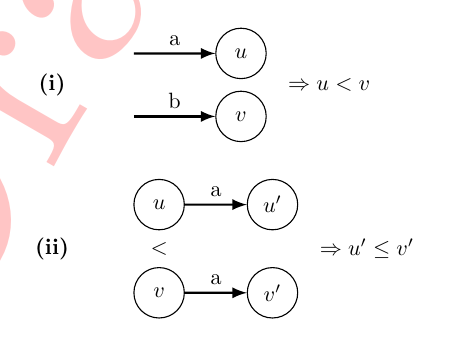
\begin{tikzpicture}[scale=0.8, transform shape,
				node distance=1.7cm,
				accepting/.style={double, fill=green!20},
				edge label/.style={font=\small, draw=none, midway}]
			% First example (i)
			\node at (-3, 0.5) {\textbf{(i)}};
			\node[circle, draw, minimum size=8mm] (u) at (0, 1) {$u$};
			\node[circle, draw, minimum size=8mm] (v) at (0, 0) {$v$};
			\draw[-latex, thick] (-1.7, 1) -- (u) node[midway, above] {a};
			\draw[-latex, thick] (-1.7, 0) -- (v) node[midway, above] {b};
			\node at (1.4, 0.5) {$\Rightarrow u < v$};

			% Second example (ii)
			\node at (-3, -2.1) {\textbf{(ii)}};
			\node[circle, draw, minimum size=8mm] (u2) at (-1.3, -1.4) {$u$};
			\node[circle, draw, minimum size=8mm] (up2) at (0.5, -1.4) {$u'$};
			\node[circle, draw, minimum size=8mm] (v2) at (-1.3, -2.8) {$v$};
			\node[circle, draw, minimum size=8mm] (vp2) at (0.5, -2.8) {$v'$};
			\draw[-latex, thick] (u2) -- (up2) node[midway, above] {a};
			\draw[-latex, thick] (v2) -- (vp2) node[midway, above] {a};
			\node at (-1.3, -2.1) {$<$};
			\node at (2, -2.1) {$\Rightarrow u' \leq v'$};
		\end{tikzpicture}

		\column{0.5\textwidth}
		\onslide<2->
		\textcolor{oiBlue}{\textbf{Wheeler DFAs (WDFAs)}}
		\begin{itemize}
			\item If all the states of a DFA are comparable it is called Wheeler DFA
		\end{itemize}
		\centering
		% Wheeler DFA example
		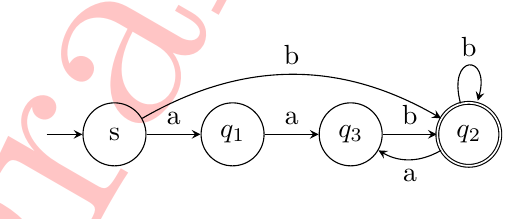
\begin{tikzpicture}[->, >=stealth, node distance=1.5cm, auto]
			\tikzset{
				state/.style={circle, draw, minimum size=0.8cm},
				accepting/.style={state, double}
			}

			\node[state, initial, initial text=] (s) at (0, 0) {s};
			\node[state] (q1) at (1.5, 0) {$q_1$};
			\node[state] (q3) at (3, 0) {$q_3$};
			\node[state, accepting] (q2) at (4.5, 0) {$q_2$};

			\path (s) edge node {a} (q1)
			(q1) edge node {a} (q3)
			(q3) edge node {b} (q2)
			(q2) edge[bend left] node {a} (q3)
			(q2) edge[loop above] node {b} (q2)
			(s) edge[bend left] node {b} (q2);

		\end{tikzpicture}

		\textbf{(i)} $s < \{q_1, q_3\} < q_2$\\
		{\small
		\hspace{0.4cm} $\epsilon$ \hspace{0.9cm} $a$ \hspace{0.9cm} $b$}


		\textbf{(ii)} $s < q_1 < q_3 < q_2$\\
		{\small
		\hspace{0.4cm} $\epsilon$ \hspace{0.4cm} $a$ \hspace{0.4cm} $a$ \hspace{0.4cm} $b$}
	\end{columns}

	\centering
	\onslide<3->
	\begin{block}{}
		This special ordering allows for highly efficient queries
	\end{block}
\end{frame}

\begin{frame}{Bipartite Representation}
	\begin{columns}[c]
		\column{0.5\textwidth}
		\centering
		\begin{figure}[t]
			\centering
			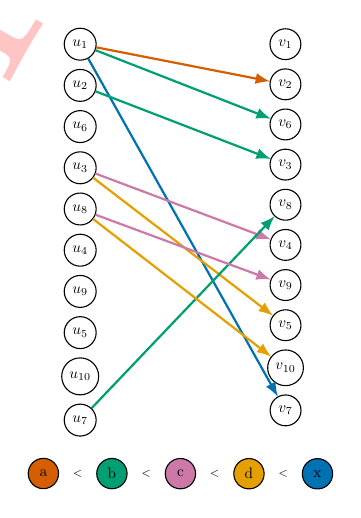
\begin{tikzpicture}[
					scale=0.55, transform shape,
					vnode/.style={circle, draw, minimum size=7mm},
					edge_label/.style={midway, font=\scriptsize}
				]
				% V_1 nodes (source)
				\node[vnode] (u1) at (0, -1.2) {$u_{1}$};
				\node[vnode, below=0.2cm of u1] (u2) {$u_{2}$};
				\node[vnode, below=0.2cm of u2] (u6) {$u_{6}$};
				\node[vnode, below=0.2cm of u6] (u3) {$u_{3}$};
				\node[vnode, below=0.2cm of u3] (u8) {$u_{8}$};
				\node[vnode, below=0.2cm of u8] (u4) {$u_{4}$};
				\node[vnode, below=0.2cm of u4] (u9) {$u_{9}$};
				\node[vnode, below=0.2cm of u9] (u5) {$u_{5}$};
				\node[vnode, below=0.2cm of u5] (u10) {$u_{10}$};
				\node[vnode, below=0.2cm of u10] (u7) {$u_{7}$};

				% V_2 nodes (destination)
				\node[vnode, right=4cm of u1] (v1) {$v_{1}$};
				\node[vnode, below=0.2cm of v1] (v2) {$v_{2}$};
				\node[vnode, below=0.2cm of v2] (v6) {$v_{6}$};
				\node[vnode, below=0.2cm of v6] (v3) {$v_{3}$};
				\node[vnode, below=0.2cm of v3] (v8) {$v_{8}$};
				\node[vnode, below=0.2cm of v8] (v4) {$v_{4}$};
				\node[vnode, below=0.2cm of v4] (v9) {$v_{9}$};
				\node[vnode, below=0.2cm of v9] (v5) {$v_{5}$};
				\node[vnode, below=0.2cm of v5] (v10) {$v_{10}$};
				\node[vnode, below=0.2cm of v10] (v7) {$v_{7}$};

				% Edges fra u_i e v_j (colori aggiornati, CVD-safe)
				\draw[-latex, oiVermillion, thick] (u1) -- (v2); \path (u1) -- (v2) node[edge_label, above] {};
				\draw[-latex, oiBlue, thick]       (u1) -- (v7); \path (u1) -- (v7) node[edge_label, above, thick] {};
				\draw[-latex, oiGreen, thick]       (u1) -- (v6); \path (u1) -- (v6) node[edge_label, above] {};

				\draw[-latex, oiGreen, thick]      (u2) -- (v3); \path (u2) -- (v3) node[edge_label, above] {};

				\draw[-latex, oiPurple, thick]     (u3) -- (v4); \path (u3) -- (v4) node[edge_label, above] {};
				\draw[-latex, oiOrange, thick]     (u3) -- (v5); \path (u3) -- (v5) node[edge_label, above] {};

				\draw[-latex, oiGreen, thick]      (u7) -- (v8); \path (u7) -- (v8) node[edge_label, above] {};
				\draw[-latex, oiPurple, thick]     (u8) -- (v9); \path (u8) -- (v9) node[edge_label, above] {};
				\draw[-latex, oiOrange, thick]     (u8) -- (v10); \path (u8) -- (v10) node[edge_label, above] {};

				\node[vnode, fill=oiVermillion, below=0.5cm of u7, xshift=-0.85cm] (a) {a};
				\node[right=0.2cm of a, font=\scriptsize] (lt1) {$<$};
				\node[vnode, fill=oiGreen, right=0.2cm of lt1] (b) {b};
				\node[right=0.2cm of b, font=\scriptsize] (lt2) {$<$};
				\node[vnode, fill=oiPurple, right=0.2cm of lt2] (c) {c};
				\node[right=0.2cm of c, font=\scriptsize] (lt3) {$<$};
				\node[vnode, fill=oiOrange, right=0.2cm of lt3] (d) {d};
				\node[right=0.2cm of d, font=\scriptsize] (lt4) {$<$};
				\node[vnode, fill=oiBlue, right=0.2cm of lt4] (x) {x};
			\end{tikzpicture}
			\caption{Bipartite representation for trie of \ref{fig:trie_example}.}
		\end{figure}
		\column{0.5\textwidth}
		\textcolor{oiBlue}{\textbf{Bipartite Representation}}
		\begin{itemize}
			\item[\checkmark] Edge labels appear in alphabetical order from top to bottom.
			\item[\checkmark] No two edges bearing the same label may cross.
		\end{itemize}
		\vspace{0.3cm}
		\centering
		\onslide<2->
		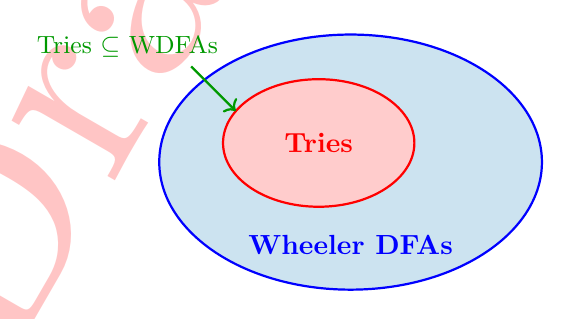
\begin{tikzpicture}[scale=0.81]
			% Wheeler DFAs circle (larger)
			\draw[thick, blue, fill=oiBlue!20] (0,0) ellipse (3cm and 2cm);
			\node[blue, font=\bfseries] at (0, -1.3) {Wheeler DFAs};

			% Tries circle (smaller, inside Wheeler DFAs)
			\draw[thick, red, fill=oiRed!20] (-0.5, 0.3) ellipse (1.5cm and 1cm);
			\node[red, font=\bfseries] at (-0.5, 0.3) {Tries};

			% Arrow showing subset relationship
			\draw[->, thick, green!60!black] (-2.5, 1.5) -- (-1.8, 0.8);
			\node[green!60!black, font=\small] at (-3.5, 1.8) {Tries $\subseteq$ WDFAs};
		\end{tikzpicture}

	\end{columns}
\end{frame}

\begin{frame}{$p$--sortable Automata: A Generalization of Wheeler Automata}
	\textcolor{oiBlue}{\textbf{Wheeler Automata}}
	\begin{columns}[c]
		\column{0.5\textwidth}
		\begin{greenblock}{Pros}
			Linear time queries
		\end{greenblock}

		\column{0.5\textwidth}
		\begin{block}{Cons}
			Very few automata are Wheeler
		\end{block}

	\end{columns}

	\vspace{0.5cm}
	\onslide<2->
	\color{oiGreen}{\textbf{Solution:}}
	\begin{itemize}
		\item Move to \textbf{partial orders}
		\item A partial order can be split in chains
		\item The minimum number of chains is the width ($p$)
	\end{itemize}
	\onslide<3->
	\color{oiVermillion}{\textbf{Important Result:}}
	\begin{itemize}
		\item Increasing $p$ can yield exponential compression~[\cite{manziniRationalConstructionWheeler2024}]
	\end{itemize}
\end{frame}

\begin{comment}
\begin{block}{\textcolor{white}{\textbf{$p$--sortable Automaton~[\cite{cotumaccio2021indexing}]}}}
	An automaton $\mathcal{A} = (Q, \Sigma, \delta, q_0, F)$ is \textbf{$\mathbf{p}$--sortable} if its states can be \textcolor{oiGreen}{\textbf{partitioned}} into $p$ subsets $\{Q_1, \dots, Q_p\}$, each admitting its own \textcolor{oiBlue}{\textbf{total order}} that satisfies the Wheeler axioms within the subset.
\end{block}

\vspace{0.2cm}
\small
\textbf{Key Insight}
\begin{itemize}
	\item \textcolor{oiPurple}{\textbf{$p = 1$:}} Standard Wheeler automaton
	      \begin{itemize}
		      \item Complete total order
		      \item Most restrictive case
	      \end{itemize}
	\item \textcolor{oiPurple}{\textbf{$p > 1$:}} Generalized structure
	      \begin{itemize}
		      \item $p$ ordered chains
		      \item Partial order flexibility
	      \end{itemize}
\end{itemize}
\end{comment}

\begin{frame}{Example: $p$--sortable Automata}
	\begin{figure}
		\centering
		\begin{subfigure}[b]{0.6\textwidth}
			\centering
			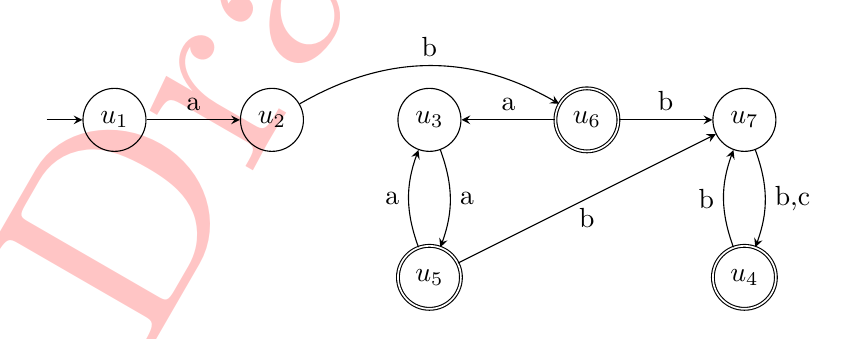
\begin{tikzpicture}[->, >=stealth, node distance=1.5cm, auto]
				\tikzset{
					state/.style={circle, draw, minimum size=0.8cm},
					accepting/.style={state, double}
				}

				\node[state, initial, initial text=] (v1) at (0,1) {$u_1$};
				\node[state] (v2) at (2,1) {$u_2$};
				\node[state] (v3) at (4,1) {$u_3$};
				\node[accepting] (v5) at (4,-1) {$u_5$};
				\node[accepting] (v6) at (6,1) {$u_6$};
				\node[state] (v7) at (8,1) {$u_7$};
				\node[accepting] (v4) at (8,-1) {$u_4$};

				\path (v1) edge node {a} (v2)
				(v2) edge [bend left=30] node[above] {b} (v6)
				(v6) edge [bend left=0] node[above] {a} (v3)
				(v3) edge [bend left=20] node[right] {a} (v5)
				(v5) edge [bend left=20] node[left] {a} (v3)
				(v5) edge node[below] {b} (v7)
				(v6) edge [bend right=0] node[above] {b} (v7)
				(v7) edge [bend left=20] node[right] {b,c} (v4)
				(v4) edge [bend left=20] node[left] {b} (v7);
			\end{tikzpicture}
			\caption{}
			\label{fig:non_wheeler_graph_example}
		\end{subfigure}%
		\hfill
		\begin{subfigure}[b]{0.35\textwidth}
			\centering
			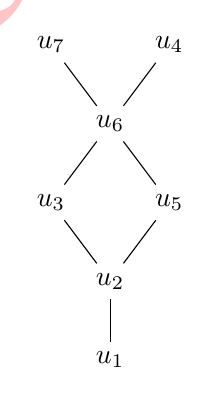
\begin{tikzpicture}
				\node (v1) at (0,0) {$u_1$};
				\node (v2) at (0,1) {$u_2$};
				\node (v3) at (-0.75,2) {$u_3$};
				\node (v5) at (0.75,2) {$u_5$};
				\node (v6) at (0,3) {$u_6$};
				\node (v4) at (0.75,4) {$u_4$};
				\node (v7) at (-0.75,4) {$u_7$};

				\draw (v1) -- (v2);
				\draw (v2) -- (v3);
				\draw (v2) -- (v5);
				\draw (v3) -- (v6);
				\draw (v5) -- (v6);
				\draw (v6) -- (v4);
				\draw (v6) -- (v7);
			\end{tikzpicture}
			\caption{}
			\label{fig:non_wheeler_graph_poset}
		\end{subfigure}
		\caption{An example of (a) a $2$--sortable DFA and (b) the corresponding Hasse diagram of its partial order.}
		\label{fig:non_wheeler_example}
	\end{figure}
\end{frame}

\begin{frame}{$p$--sortable Automata Index~[\cite{cotumaccio2021indexing}]}

	\begin{block}{\textcolor{white}{\textbf{Main Result}}}
		There exists a \textcolor{oiGreen}{\textbf{compressed data structure}} for $p$-sortable automata that supports \textcolor{oiPurple}{\textbf{subpath queries}}.
	\end{block}

	\vspace{0.3cm}
	\onslide<2->
	\textcolor{oiRed}{\textbf{Key Properties}}
	\begin{itemize}
		\item \textbf{Efficiency:} Efficient subpath query time
		\item \textbf{Generality:} Works for both DFA and NFA
		\item \textbf{Scalability:} Performance and space depend on $p$
	\end{itemize}
\end{frame}

\begin{comment}
\begin{frame}{XBWT (Extended Burrows–Wheeler Transform)}
	\begin{itemize}
		\item Extends the classic BWT from strings to labeled trees.
		\item Encodes the tree as two arrays:
		      \begin{itemize}
			      \item $S_\alpha$: node labels
			      \item $S_{last}$: structure bits
		      \end{itemize}
		\item Enables compressed storage and prefix queries.
	\end{itemize}
	\centering
	% \includegraphics[width=0.8\textwidth]{fig_xbwt_example.png}
	\small
	The children of each node form a contiguous block in $S_\alpha$.
\end{frame}
\end{comment}

% === PROPOSED METHOD ===
\fancysectionframe{Proposed Tries Compression Scheme}

\section{Proposed Compression Scheme}
\begin{frame}{Our Approach}
	\begin{columns}[t]
		\column{0.5\textwidth}
		\begin{block}{\textcolor{white}{\textbf{Partial Minimization Strategy}}}
			Produce a \textcolor{oiGreen}{\textbf{smaller, equivalent automaton}} that remains \textcolor{oiBlue}{\textbf{indexable}} by allowing \textcolor{oiRed}{\textbf{controlled partial merging}} of equivalent subtrees.
		\end{block}

		\column{0.5\textwidth}
		\begin{block}{\textcolor{white}{\textbf{Result}}}
			\centering
			\textbf{Partial Minimization} \\
			$\Downarrow$ \\
			\textbf{$\mathbf{p}$--sortable automata}

			\vspace{0.3cm}
			\tiny
			\textit{Optimal balance: compression + query efficiency}
		\end{block}
	\end{columns}
	\vspace{0.5cm}
	\onslide<2->
	\textbf{\textcolor{oiBlue}{Key Benefits}}
	\begin{itemize}
		\item \textbf{Space:} Significant memory reduction
		\item \textbf{Time:} Efficient query processing
		\item \textbf{Flexibility:} Adjustable compression level
	\end{itemize}
\end{frame}

\begin{comment}
\begin{frame}{The Intuition}
	\begin{itemize}
		\item Parameter $p$ interpolates between the two extremes:
		      \begin{itemize}
			      \item $p=1$: Wheeler graph $\Rightarrow$ maximum indexability, less compression.
			      \item $p \to \infty$: more compression, less indexability.
		      \end{itemize}
		\item Increasing $p$ improves compression but complicates indexing.
	\end{itemize}
	\vspace{0.3cm}
	\centering
	% \includegraphics[width=0.65\textwidth]{fig_psortable_graph.png}
	\small
	Example of a 2–sortable automaton: partial merging with preserved order.
\end{frame}
\end{comment}

\begin{frame}{Compression Pipeline}
	\centering
	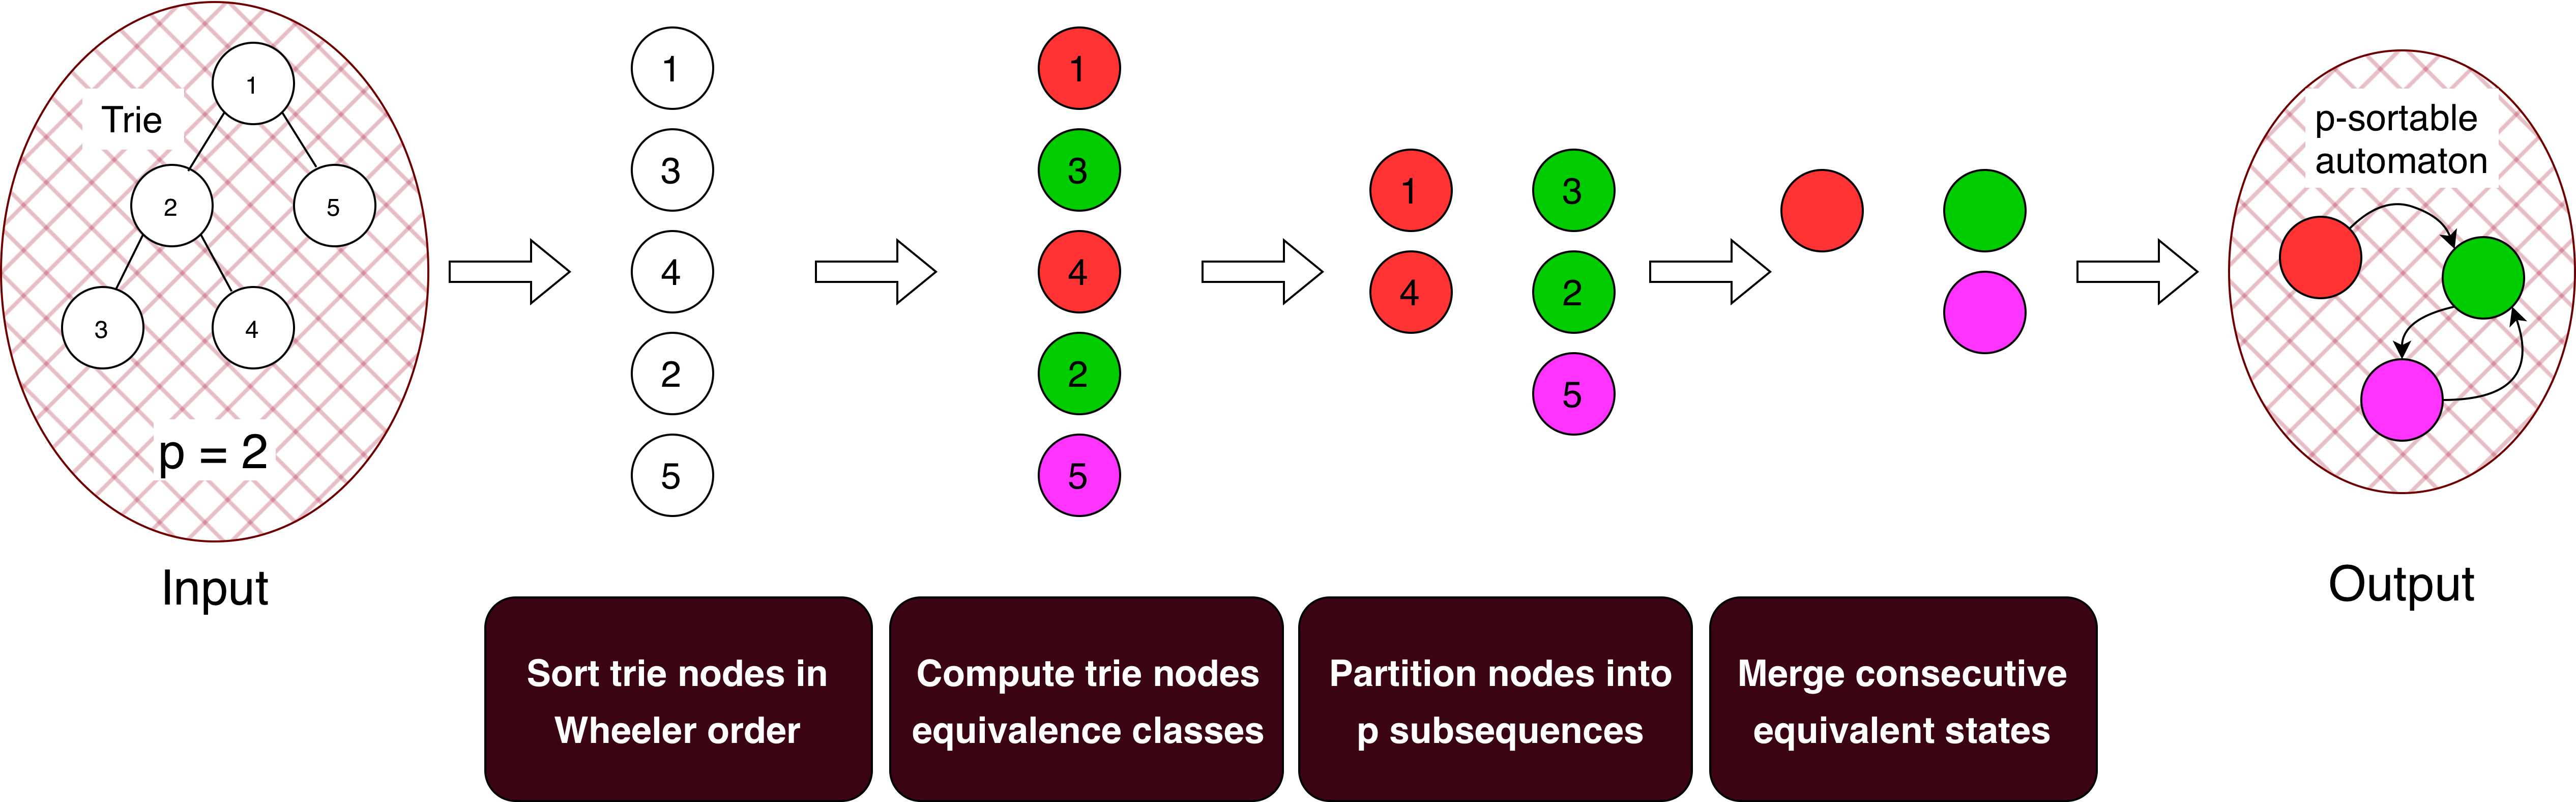
\includegraphics[width=1\textwidth]{img/pipeline.png}
\end{frame}

\begin{frame}{String Partitioning Problem}
	\begin{block}{Run}
		\textcolor{oiBlue}{\textbf{Maximal contiguous subsequence}} of identical characters within $s$.
	\end{block}
	\small
	\[
		s = \texttt{ABDCCDDDDB}
	\]

	\vspace{0.3cm}
	\centering
	\begin{figure}[t]
		\centering
		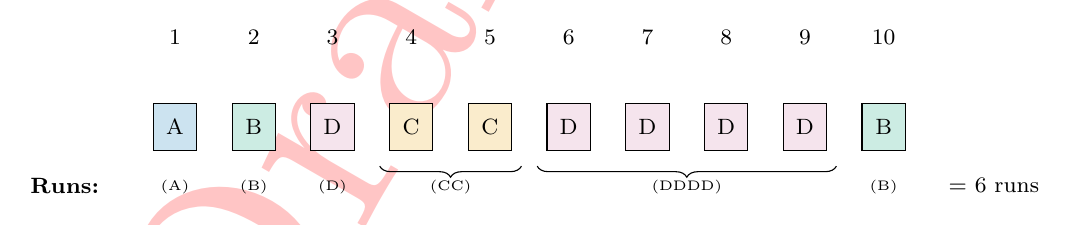
\begin{tikzpicture}[
				every node/.style={font=\footnotesize, inner sep=1pt},
				box/.style={draw, minimum width=0.55cm, minimum height=0.6cm, align=center}
			]

			% Positions
			\foreach \i in {1,...,10} {
					\node[above=2mm] (p\i) at (\i,0) {\i};
				}

			% Characters (colored by partition)
			\node[box, fill=oiBlue!20] (c1) at (1, -0.8) {A};
			\node[box, fill=oiGreen!20] (c2) at (2, -0.8) {B};
			\node[box, fill=oiPurple!20] (c3) at (3, -0.8) {D};
			\node[box, fill=oiOrange!20] (c4) at (4, -0.8) {C};
			\node[box, fill=oiOrange!20] (c5) at (5, -0.8) {C};
			\node[box, fill=oiPurple!20] (c6) at (6, -0.8) {D};
			\node[box, fill=oiPurple!20] (c7) at (7, -0.8) {D};
			\node[box, fill=oiPurple!20] (c8) at (8, -0.8) {D};
			\node[box, fill=oiPurple!20] (c9) at (9, -0.8) {D};
			\node[box, fill=oiGreen!20] (c10) at (10, -0.8) {B};

			% Brackets for runs
			\node at (-0.4, -1.55) {\textbf{Runs:}};
			\draw[decorate, decoration={brace, amplitude=4pt}, yshift=-0.2cm]
			(1, -1.1) -- (1, -1.1) node[midway, below=4pt] {\tiny (A)};
			\draw[decorate, decoration={brace, amplitude=4pt}, yshift=-0.2cm]
			(2, -1.1) -- (2, -1.1) node[midway, below=4pt] {\tiny (B)};
			\draw[decorate, decoration={brace, amplitude=4pt}, yshift=-0.2cm]
			(3, -1.1) -- (3, -1.1) node[midway, below=4pt] {\tiny (D)};
			\draw[decorate, decoration={brace, amplitude=4pt, mirror}, yshift=-0.2cm]
			(3.6, -1.1) -- (5.4, -1.1) node[midway, below=4pt] {\tiny (CC)};
			\draw[decorate, decoration={brace, amplitude=4pt, mirror}, yshift=-0.2cm]
			(5.6, -1.1) -- (9.4, -1.1) node[midway, below=4pt] {\tiny (DDDD)};
			\draw[decorate, decoration={brace, amplitude=4pt}, yshift=-0.2cm]
			(10, -1.1) -- (10, -1.1) node[midway, below=4pt] {\tiny (B)};

			\node at (11.4, -1.55) {= 6 runs};
		\end{tikzpicture}
		\vspace{0.5cm}
		\caption{Initial runs of the string induced by the equivalence class of the sorted trie nodes in \ref{fig:trie_example}.}
		\label{fig:string_example}
	\end{figure}
\end{frame}

\begin{frame}{String Partitioning Problem}
	\begin{block}{String Partitioning Problem}
		Partition $s$ into $p$ subsequences \textcolor{oiBlue}{\textbf{minimizing}} number of \textcolor{oiRed}{\textbf{runs}}.
	\end{block}

	\vspace{0.1cm}
	\onslide<2->
	\begin{itemize}
		\item Reducible to: \textcolor{oiGreen}{\textbf{Minimum Weight Perfect Bipartite Matching (MWPBM)}}
	\end{itemize}

	\vspace{0.2cm}

	\begin{figure}[H]
		\centering
		\begin{subfigure}[b]{0.45\textwidth}
			\centering
			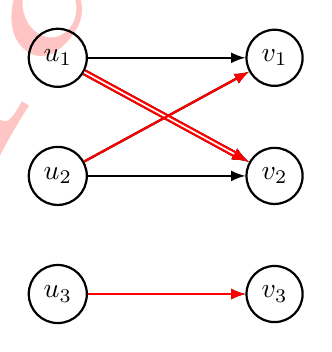
\begin{tikzpicture}[node distance={15mm}, thick, auto=center, main/.style = {draw, circle}]
				\node[main] (u1) {$u_1$};
				\node[main] (u2) [below of=u1] {$u_2$};
				\node[main] (u3) [below of=u2] {$u_3$};
				\node[main] (v1) [right=2cm of u1] {$v_1$};
				\node[main] (v2) [below of=v1] {$v_2$};
				\node[main] (v3) [below of=v2] {$v_3$};
				\draw[-latex] (u1) -- (v1);
				\draw[-latex, double] (u1) -- (v2);
				\draw[-latex] (u2) -- (v1);
				\draw[-latex] (u2) -- (v2);
				\draw[-latex] (u3) -- (v3);
				\draw[-latex, double, red] (u1) -- (v2);
				\draw[-latex, red] (u2) -- (v1);
				\draw[-latex, red] (u3) -- (v3);
			\end{tikzpicture}
			\caption{Non-min. weight perfect matching (tot 4)}
			\label{fig:mwpbm_non_perfect}
		\end{subfigure}
		\hfill
		\begin{minipage}[b]{0.08\textwidth}
			\centering

			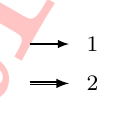
\begin{tikzpicture}
				\draw[-latex] (0,0.5) -- (0.5,0.5);
				\node[right] at (0.6,0.5) {\footnotesize 1};
				\draw[-latex, double] (0,0) -- (0.5,0);
				\node[right] at (0.6,0) {\footnotesize 2};
			\end{tikzpicture}
			\vspace{1.8cm}
		\end{minipage}
		\hfill
		\begin{subfigure}[b]{0.45\textwidth}
			\centering
			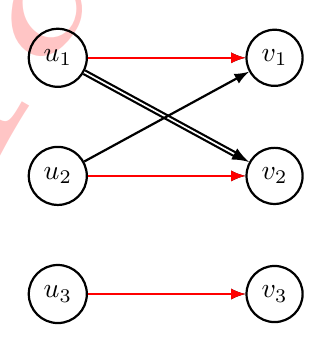
\begin{tikzpicture}[node distance={15mm}, thick, auto=center, main/.style = {draw, circle}]
				\node[main] (u1) {$u_1$};
				\node[main] (u2) [below of=u1] {$u_2$};
				\node[main] (u3) [below of=u2] {$u_3$};
				\node[main] (v1) [right=2cm of u1] {$v_1$};
				\node[main] (v2) [below of=v1] {$v_2$};
				\node[main] (v3) [below of=v2] {$v_3$};
				\draw[-latex] (u1) -- (v1);
				\draw[-latex, double] (u1) -- (v2);
				\draw[-latex] (u2) -- (v1);
				\draw[-latex] (u2) -- (v2);
				\draw[-latex] (u3) -- (v3);
				\draw[-latex, red] (u1) -- (v1);
				\draw[-latex, red] (u2) -- (v2);
				\draw[-latex, red] (u3) -- (v3);
			\end{tikzpicture}
			\caption{Min. weight perfect matching (tot 3)}
			\label{fig:mwpbm_perfect}
		\end{subfigure}
		\label{fig:mwpbm_example}
	\end{figure}
\end{frame}

\begin{frame}{Reduction to Bipartite Graph Matching}
	\centering
	\vspace{0.2cm}
	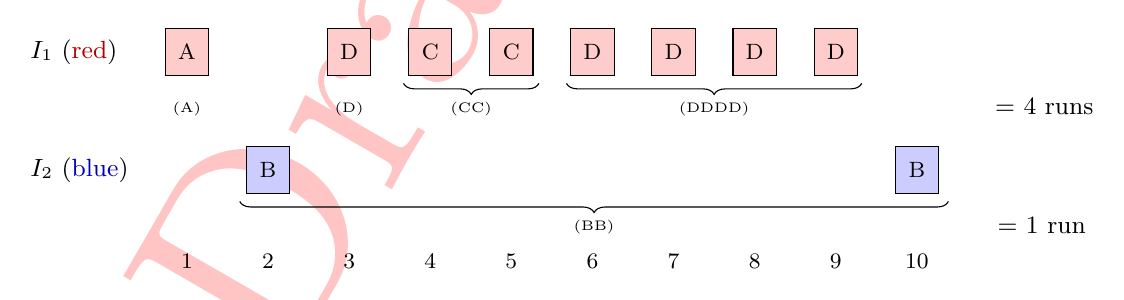
\begin{tikzpicture}[
			every node/.style={font=\footnotesize, inner sep=1pt},
			box/.style={draw, minimum width=0.55cm, minimum height=0.6cm, align=center}
		]

		% Indices
		\foreach \i in {1,...,10} {
				\node[above=2mm] at (\i*1.03, -3.8) {\i};
			}

		% --- Partition s2 (red) ---
		\node[anchor=west, font=\small] at (-1, -0.8) {$I_1$ (\textcolor{red!70!black}{red})};
		\node[box, fill=red!20] (r1)  at (1*1.03, -0.8) {A};
		\node[box, fill=red!20] (r2)  at (3*1.03, -0.8) {D};
		\node[box, fill=red!20] (r3)  at (4*1.03, -0.8) {C};
		\node[box, fill=red!20] (r4)  at (5*1.03, -0.8) {C};
		\node[box, fill=red!20] (r5)  at (6*1.03, -0.8) {D};
		\node[box, fill=red!20] (r6)  at (7*1.03, -0.8) {D};
		\node[box, fill=red!20] (r7)  at (8*1.03, -0.8) {D};
		\node[box, fill=red!20] (r8)  at (9*1.03, -0.8) {D};

		\draw[decorate, decoration={brace, amplitude=4pt}, yshift=-0.2cm]
		(1.03, -1.05) -- (1.03, -1.05) node[midway, below=4pt] {\tiny (A)};
		\draw[decorate, decoration={brace, amplitude=4pt}, yshift=-0.2cm]
		(3.09, -1.05) -- (3.09, -1.05) node[midway, below=4pt] {\tiny (D)};
		\draw[decorate, decoration={brace, amplitude=4pt, mirror}, yshift=-0.2cm]
		(3.78, -1) -- (5.5, -1) node[midway, below=0.2cm] {\tiny (CC)};
		\draw[decorate, decoration={brace, amplitude=4pt, mirror}, yshift=-0.2cm]
		(5.85, -1) -- (9.6, -1) node[midway, below=0.2cm] {\tiny (DDDD)};

		\node[font=\small, right=1.7cm of r8, yshift=-0.7cm] {= 4 runs};

		% --- Partition s1 (blue) ---
		\node[anchor=west, font=\small] at (-1, -2.3) {$I_2$ (\textcolor{blue!70!black}{blue})};
		\node[box, fill=blue!20] (b1) at (2*1.03, -2.3) {B};
		\node[box, fill=blue!20] (b2) at (10*1.03, -2.3) {B};

		\draw[decorate, decoration={brace, amplitude=4pt, mirror}]
		(1.7, -2.7) -- (10.7, -2.7) node[midway, below=0.2cm] {\tiny (BB)};

		\node[font=\small, right=0.7cm of b2, yshift=-0.7cm] {= 1 run};
	\end{tikzpicture}

	\begin{figure}[t]
		\centering
		\begin{tikzpicture}[
				scale=0.6, transform shape,
				vnode/.style={circle, draw, minimum size=9mm},
				edge_label/.style={midway, font=\scriptsize}
			]
			% Source nodes
			\node[vnode, fill=oiGreen] (s1) at (-3.2, 0) {$s_{1}$};
			\node[vnode, fill=oiGreen] (s2) at (-1.6, 0) {$s_{2}$};

			% V_1 nodes (source) - horizontal layout
			\node[vnode] (u1) at (0, 0) {A};
			\node[vnode, right=0.8cm of u1] (u2) {B};
			\node[vnode, right=0.8cm of u2] (u6) {D};
			\node[vnode, right=0.8cm of u6] (u3) {C};
			\node[vnode, right=0.8cm of u3] (u8) {C};
			\node[vnode, right=0.8cm of u8] (u4) {D};
			\node[vnode, right=0.8cm of u4] (u9) {D};
			\node[vnode, right=0.8cm of u9] (u5) {D};
			\node[vnode, right=0.8cm of u5] (u10) {D};
			\node[vnode, right=0.8cm of u10] (u7) {B};

			% V_2 nodes (destination) - horizontal layout below
			\node[vnode, below=3cm of u1] (v1) {A};
			\node[vnode, right=0.8cm of v1] (v2) {B};
			\node[vnode, right=0.8cm of v2] (v6) {D};
			\node[vnode, right=0.8cm of v6] (v3) {C};
			\node[vnode, right=0.8cm of v3] (v8) {C};
			\node[vnode, right=0.8cm of v8] (v4) {D};
			\node[vnode, right=0.8cm of v4] (v9) {D};
			\node[vnode, right=0.8cm of v9] (v5) {D};
			\node[vnode, right=0.8cm of v5] (v10) {D};
			\node[vnode, right=0.8cm of v10] (v7) {B};

			% Destination nodes
			\node[vnode, fill=oiVermillion, right=1.3cm of v10] (d1) at (v7) {$d_{1}$};
			\node[vnode, fill=oiVermillion, right=0.8cm of d1] (d2) {$d_{2}$};

			% Light grey edges (drawn first, will appear behind colored edges)
			\draw[-latex, oiLightGrey] (s1) -- (v2);
			\draw[-latex, oiLightGrey] (s1) -- (v3);
			\draw[-latex, oiLightGrey] (s1) -- (v4);
			\draw[-latex, oiLightGrey] (s1) -- (v5);
			\draw[-latex, oiLightGrey] (s1) -- (v6);
			\draw[-latex, oiLightGrey] (s1) -- (v7);
			\draw[-latex, oiLightGrey] (s1) -- (v8);
			\draw[-latex, oiLightGrey] (s1) -- (v9);
			\draw[-latex, oiLightGrey] (u9) -- (v10);
			\draw[-latex, oiLightGrey] (u1) -- (v2);
			\draw[-latex, oiLightGrey] (u1) -- (v3);
			\draw[-latex, oiLightGrey] (u1) -- (v8);
			\draw[-latex, oiLightGrey] (u1) -- (v4);
			\draw[-latex, oiLightGrey] (u1) -- (v9);
			\draw[-latex, oiLightGrey] (u1) -- (v5);
			\draw[-latex, oiLightGrey] (u1) -- (v10);
			\draw[-latex, oiLightGrey] (u1) -- (v7);
			\draw[-latex, oiLightGrey] (u2) -- (v6);
			\draw[-latex, oiLightGrey] (u2) -- (v3);
			\draw[-latex, oiLightGrey] (u2) -- (v8);
			\draw[-latex, oiLightGrey] (u2) -- (v4);
			\draw[-latex, oiLightGrey] (u2) -- (v9);
			\draw[-latex, oiLightGrey] (u2) -- (v5);
			\draw[-latex, oiLightGrey] (u2) -- (v10);
			\draw[-latex, oiLightGrey] (u6) -- (v8);
			\draw[-latex, oiLightGrey] (u6) -- (v4);
			\draw[-latex, oiLightGrey] (u6) -- (v9);
			\draw[-latex, oiLightGrey] (u6) -- (v5);
			\draw[-latex, oiLightGrey] (u6) -- (v10);
			\draw[-latex, oiLightGrey] (u6) -- (v7);
			\draw[-latex, oiLightGrey] (u3) -- (v4);
			\draw[-latex, oiLightGrey] (u3) -- (v9);
			\draw[-latex, oiLightGrey] (u3) -- (v5);
			\draw[-latex, oiLightGrey] (u3) -- (v10);
			\draw[-latex, oiLightGrey] (u3) -- (v7);
			\draw[-latex, oiLightGrey] (u8) -- (v9);
			\draw[-latex, oiLightGrey] (u8) -- (v5);
			\draw[-latex, oiLightGrey] (u8) -- (v10);
			\draw[-latex, oiLightGrey] (u8) -- (v7);
			\draw[-latex, oiLightGrey] (u4) -- (v5);
			\draw[-latex, oiLightGrey] (u4) -- (v10);
			\draw[-latex, oiLightGrey] (u4) -- (v7);
			\draw[-latex, oiLightGrey] (u9) -- (v10);
			\draw[-latex, oiLightGrey] (u9) -- (v7);
			\draw[-latex, oiLightGrey] (u5) -- (v7);
			\draw[-latex, oiLightGrey] (u10) -- (v7);
			\draw[-latex, oiLightGrey] (s2) -- (v1);
			\draw[-latex, oiLightGrey] (s2) -- (v3);
			\draw[-latex, oiLightGrey] (s2) -- (v4);
			\draw[-latex, oiLightGrey] (s2) -- (v5);
			\draw[-latex, oiLightGrey] (s2) -- (v6);
			\draw[-latex, oiLightGrey] (s2) -- (v7);
			\draw[-latex, oiLightGrey] (s2) -- (v8);
			\draw[-latex, oiLightGrey] (s2) -- (v9);
			\draw[-latex, oiLightGrey] (s2) -- (v10);

			% Colored edges (drawn last, will appear on top)
			\draw[-latex, oiRed, thick] (s1) -- (v1);
			\draw[-latex, oiRed, thick] (u1) -- (v6);
			\draw[-latex, oiBlue, thick] (u2) -- (v7);
			\draw[-latex, oiRed, thick] (u6) -- (v3);
			\draw[-latex, oiRed, thick] (u3) -- (v8);
			\draw[-latex, oiRed, thick] (u8) -- (v4);
			\draw[-latex, oiRed, thick] (u4) -- (v9);
			\draw[-latex, oiRed, thick] (u9) -- (v5);
			\draw[-latex, oiRed, thick] (u5) -- (v10);
			\draw[-latex, oiBlue, thick] (s2) -- (v2);

			% Edges from all u_x nodes to destination nodes
			\draw[-latex, oiLightGrey] (u1) -- (d1);
			\draw[-latex, oiLightGrey] (u1) -- (d2);
			\draw[-latex, oiLightGrey] (u2) -- (d1);
			\draw[-latex, oiLightGrey] (u2) -- (d2);
			\draw[-latex, oiLightGrey] (u3) -- (d1);
			\draw[-latex, oiLightGrey] (u3) -- (d2);
			\draw[-latex, oiLightGrey] (u4) -- (d1);
			\draw[-latex, oiLightGrey] (u4) -- (d2);
			\draw[-latex, oiLightGrey] (u5) -- (d1);
			\draw[-latex, oiLightGrey] (u5) -- (d2);
			\draw[-latex, oiLightGrey] (u6) -- (d1);
			\draw[-latex, oiLightGrey] (u6) -- (d2);
			\draw[-latex, oiLightGrey] (u7) -- (d1);
			\draw[-latex, oiBlue, thick] (u7) -- (d2);
			\draw[-latex, oiLightGrey] (u8) -- (d1);
			\draw[-latex, oiLightGrey] (u8) -- (d2);
			\draw[-latex, oiLightGrey] (u9) -- (d1);
			\draw[-latex, oiLightGrey] (u9) -- (d2);
			\draw[-latex, oiRed, thick] (u10) -- (d1);
			\draw[-latex, oiLightGrey] (u10) -- (d2);

			% Legend
			%\node at (8.6, -5) {
			%	\begin{tikzpicture}[baseline=(current bounding box.center)]
			%		\draw[-latex, oiBlue, thick] (0, 0) -- (0.8, 0);
			%		\node[above] at (0.4, 0) {\small 1};
			%		\draw[-latex, oiRed, thick] (3, 0) -- (3.8, 0);
			%		\node[above] at (3.4, 0) {\small 0};
			%	\end{tikzpicture}
			%};
		\end{tikzpicture}
		\vspace{0.1cm}
		\caption{Reduction for string in \ref{fig:string_example}. The minimum weight perfect matching is highlighted.}
	\end{figure}
\end{frame}

\begin{frame}{Reduction to Bipartite Graph Matching}
	\textcolor{oiRed}{\textbf{Graph Construction}}
	\begin{itemize}
		\item \textbf{Nodes:} Correspond to string characters
		\item \textbf{Edges:} Encode successor relation
		      \begin{itemize}
			      \item Weight represents transition cost: 1 if characters differ, 0 otherwise
		      \end{itemize}
		\item \textbf{Complexity:} $\mathcal{O}(n^2)$ edges in current version
		      \begin{itemize}
			      \item Can be improved to $\mathcal{O}(np)$
		      \end{itemize}
	\end{itemize}

	\vspace{0.2cm}
	\onslide<2->
	\begin{block}{\textcolor{white}{\textbf{Optimization Objective}}}
		Solving \textbf{MWPBM} yields an \textcolor{oiBlue}{\textbf{optimal partition}} minimizing the \textcolor{oiBlue}{\textbf{total number of runs}} across all subsequences.
	\end{block}
\end{frame}

% === IMPLEMENTATION AND RESULTS ===
\fancysectionframe{Implementation and Experiments}

\section{Implementation and Experiments}
\begin{frame}{Experimental Setup}
	\begin{itemize}
		\item \textcolor{oiBlue}{\textbf{Implementation}:} C++ for high performance and efficiency
		\item \textcolor{oiGreen}{\textbf{Hardware}:} Apple M4 Pro with 24 GB RAM
		\item \textcolor{oiRed}{\textbf{Dataset}:} Synthetic tries with controlled size and repetitiveness
	\end{itemize}
\end{frame}

\begin{frame}{Experimental Results (1)}
	\begin{itemize}
		\item Each trie in the dataset contains \textcolor{oiBlue}{\textbf{100,000 nodes}}
		\item Increasing $p$ from 1 to 2 \textcolor{oiRed}{\textbf{halves the number of states}}
		\item Compression ratio \textcolor{oiGreen}{\textbf{approaches the minimal number of states}}
	\end{itemize}
	\centering
	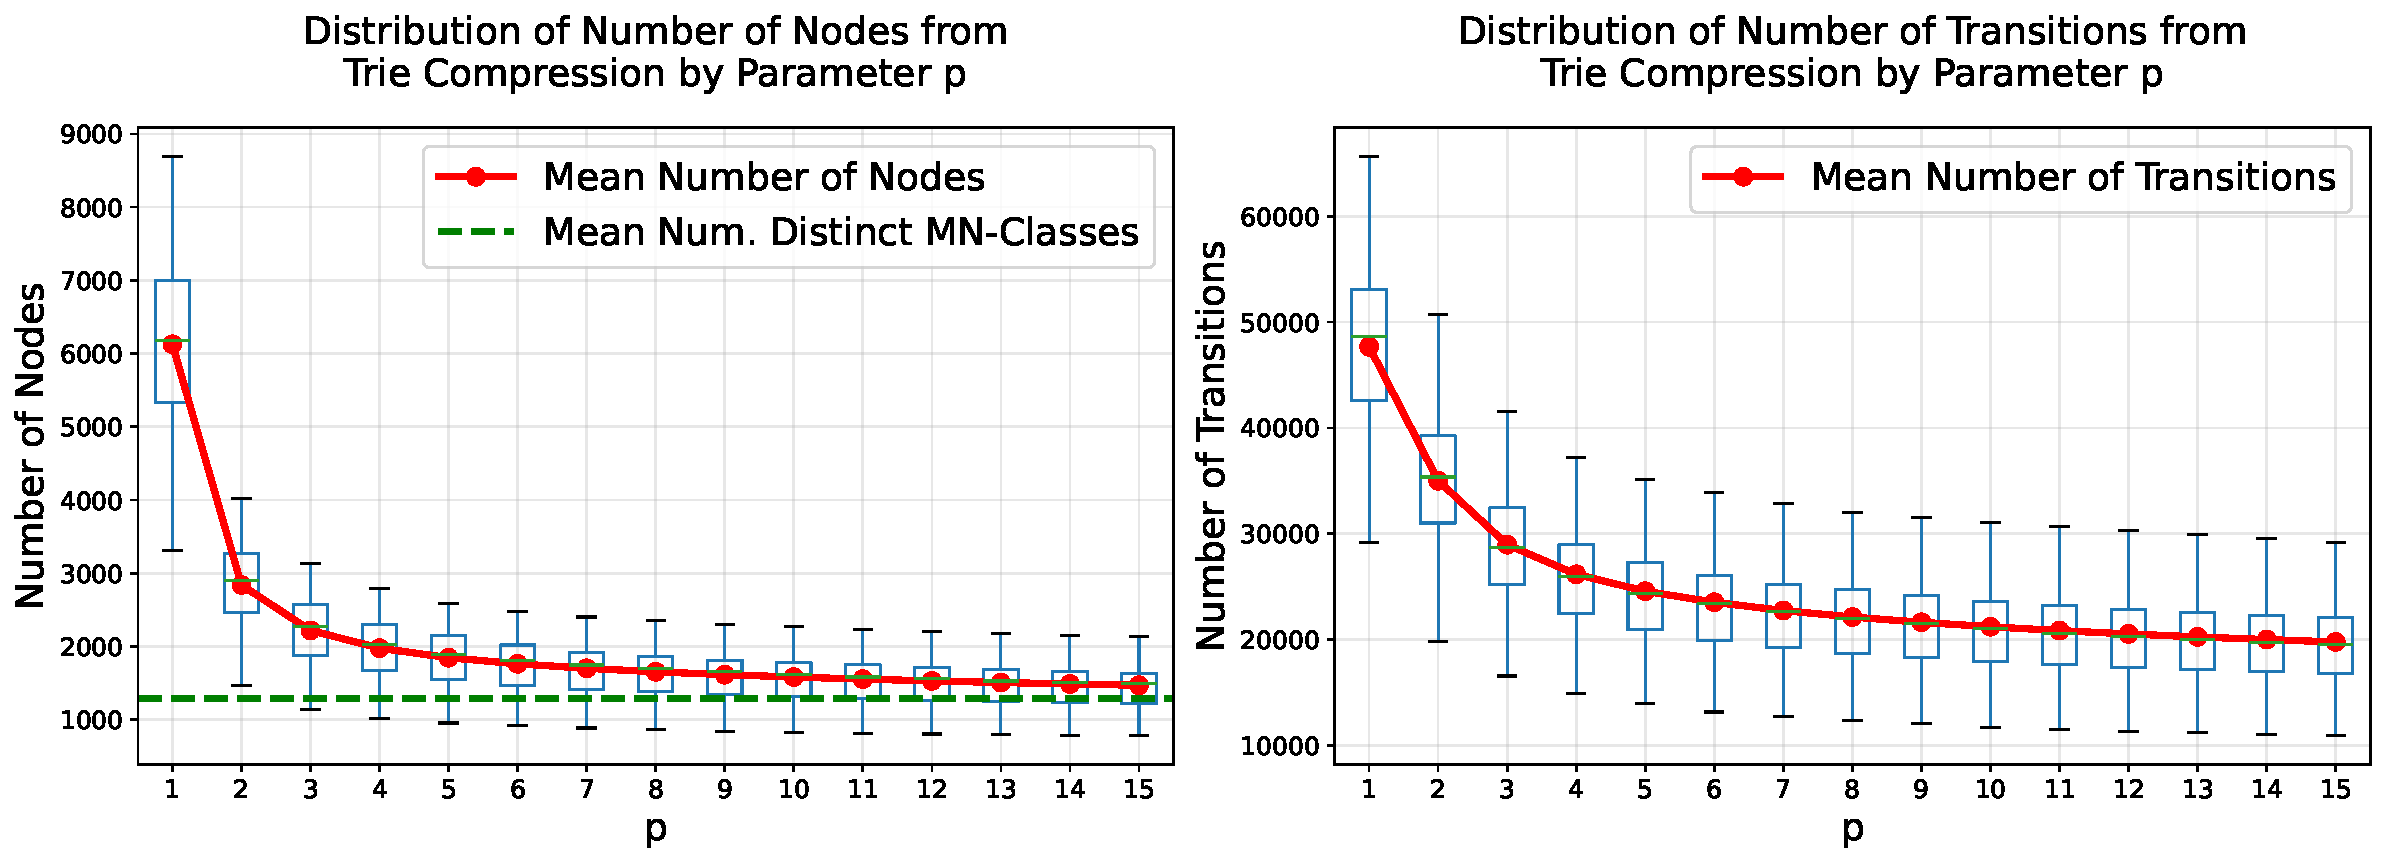
\includegraphics[width=1\textwidth]{img/tree_compression_analysis.pdf}
\end{frame}

\begin{frame}{Experimental Results (2)}
	\begin{itemize}
		\item Each trie in the datasets contains \textcolor{oiBlue}{\textbf{100,000 nodes}}
		\item \textcolor{oiRed}{\textbf{Tries with high repetitiveness compress better}} independently of $p$
	\end{itemize}
	\centering
	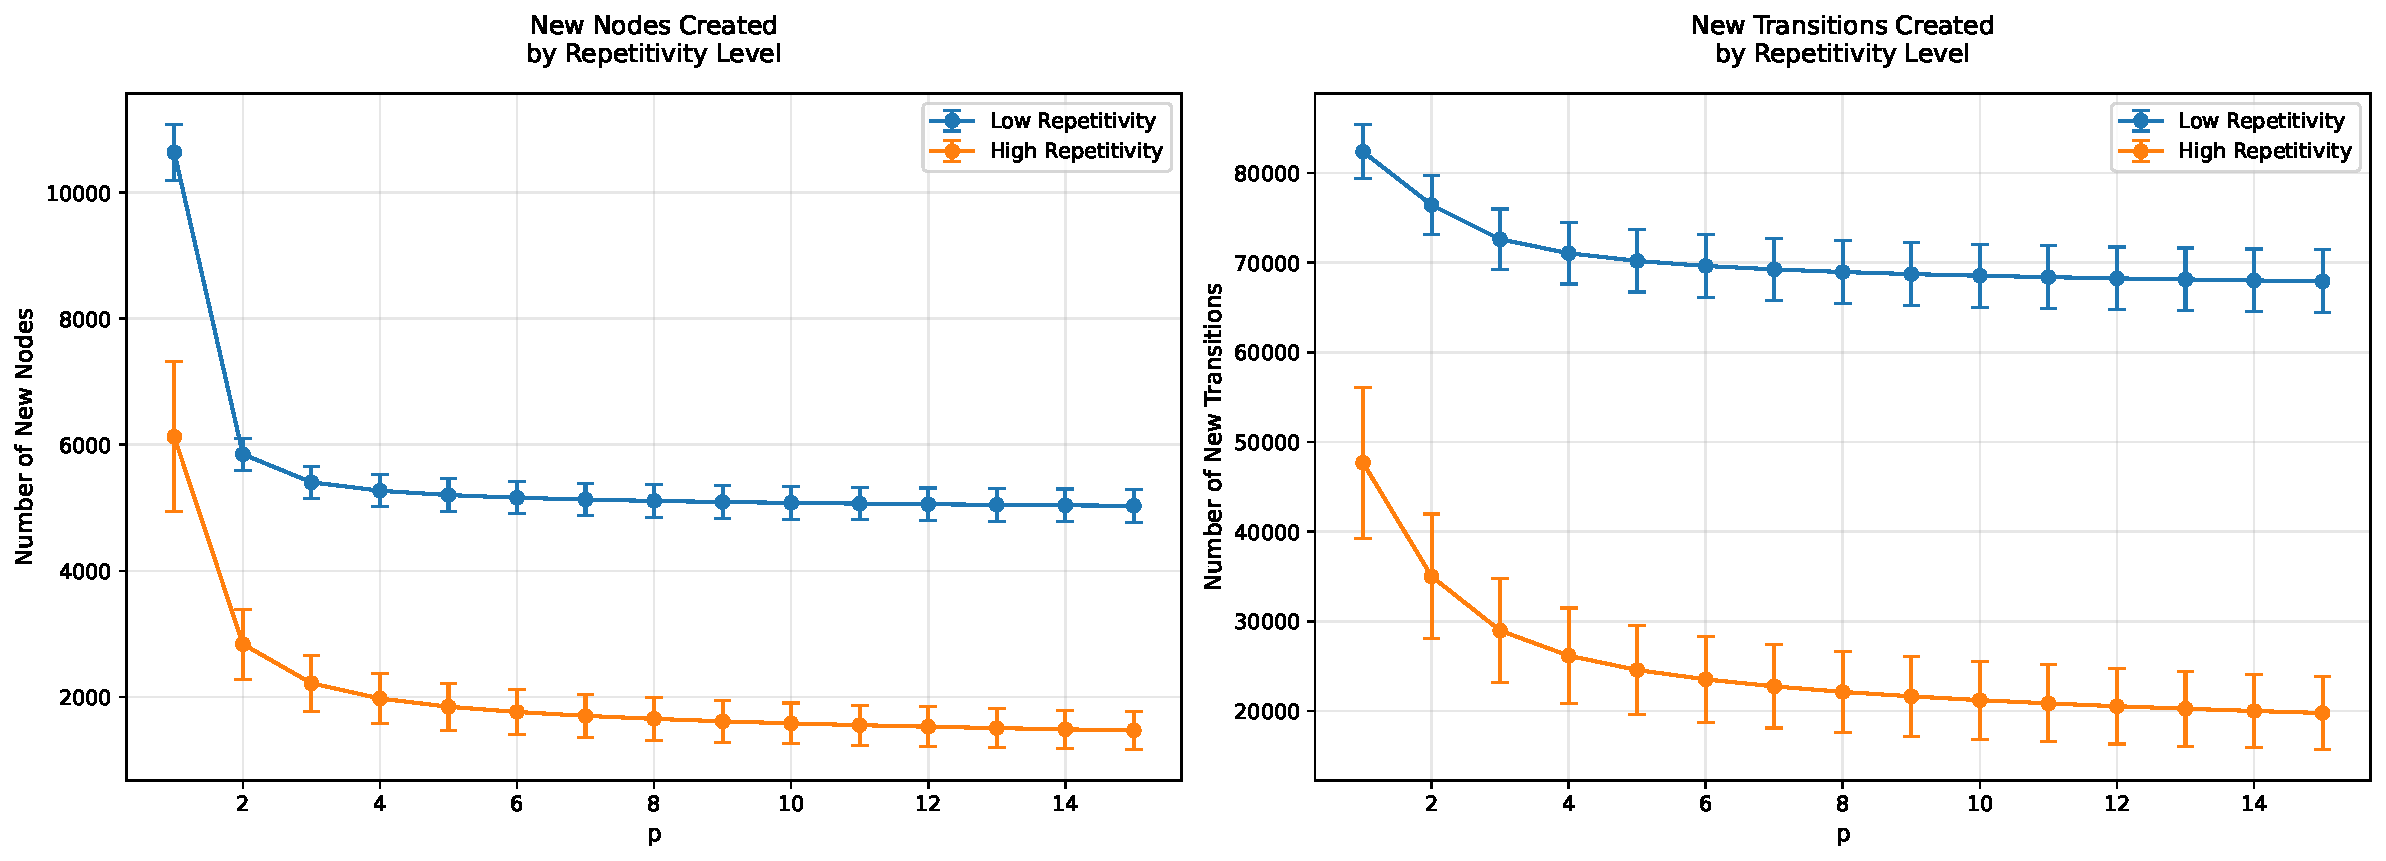
\includegraphics[width=1\textwidth]{img/high_low_comparison.pdf}
\end{frame}

% === CONCLUSIONS ===
\fancysectionframe{Conclusions}

\section{Conclusions}
\begin{frame}{Conclusions}
	\begin{block}{Our Contribution}
		Introduced a new compressed index for tries
	\end{block}
	\vspace{0.3cm}
	\onslide<2->
	\textcolor{oiBlue}{\textbf{Key Achievements}:}
	\begin{itemize}
		\item \textbf{Memory Efficiency}: Significant space reduction on repetitive datasets
		\item \textbf{Query Performance}: Maintains efficient sub-path queries
		\item \textbf{Adaptability}: Tunable compression via parameter $p$
	\end{itemize}
\end{frame}

\begin{frame}{Future Works}
	\begin{itemize}
		\item<1-> \textcolor{oiRed}{\textbf{Scalability}:} Develop more efficient solutions for large-scale applications.
		\item<2-> \textcolor{oiBlue}{\textbf{DFA Construction}:} Always get a $p$--sortable DFA from the compression scheme.
		\item<3-> \textcolor{oiOrange}{\textbf{DFA Minimality}:} Guarantee the minimality of the constructed $p$--sortable DFA.
	\end{itemize}

	\vspace{1cm}
	\textbf{The research and development of these future works will be continued during the author's PhD program.}
\end{frame}

\begin{frame}
	\centering
	\Huge
	Thank you for your attention!

	\vspace{1cm}
	\Large
	Questions?
\end{frame}

\begin{frame}{Example: $\mathcal{O}(n^2)$ MWPBM Reduction}
	\centering
	\begin{figure}[H]
		\centering
		\scalebox{0.9}{%
			\begin{minipage}{\textwidth}
				\centering
				\tikzset{main/.style = {draw, circle, thick, minimum size=8mm, inner sep=0pt}}
				\begin{subfigure}[b]{0.3\textwidth}
					\centering
					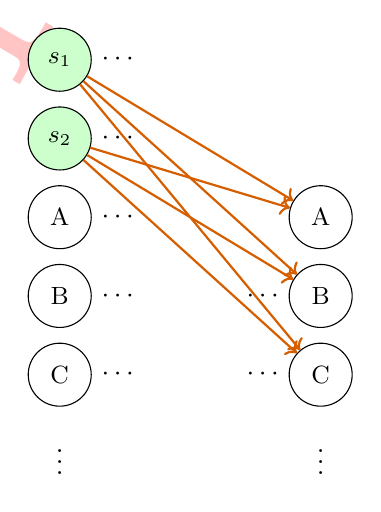
\begin{tikzpicture}[node distance=10mm, auto=center]
						\tikzstyle{main} = [circle, draw, minimum size=0.8cm, font=\small]
						\tikzstyle{source} = [circle, draw, minimum size=0.8cm, font=\small, fill=green!20]
						\tikzstyle{dest} = [circle, draw, minimum size=0.8cm, font=\small, fill=blue!20]

						% Left column (sources)
						\node[source] (1s) {$s_1$};
						\node[right=0cm of 1s] {$\cdots$};
						\node[source] (2s) [below of=1s] {$s_2$};
						\node[right=0cm of 2s] {$\cdots$};
						\node[main] (3s) [below of=2s] {A};
						\node[right=0cm of 3s] {$\cdots$};
						\node[main] (4s) [below of=3s] {B};
						\node[right=0cm of 4s] {$\cdots$};
						\node[main] (5s) [below of=4s] {C};
						\node[right=0cm of 5s] {$\cdots$};
						\node (dots_s) [below of=5s] {\vdots}; % Vertical dots

						% Right column (destinations)
						\node[main] (1d) [right=2.5cm of 3s] {A};
						\node[main] (2d) [below of=1d] {B};
						\node[left=0cm of 2d] {$\cdots$};
						\node[main] (3d) [below of=2d] {C};
						\node[left=0cm of 3d] {$\cdots$};
						\node (dots_d) [below of=3d] {\vdots}; % Vertical dots

						% Arrows
						\draw[oiVermillion, ->, thick] (1s) -- (1d);
						\draw[oiVermillion, ->, thick] (1s) -- (2d);
						\draw[oiVermillion, ->, thick] (1s) -- (3d);
						\draw[oiVermillion, ->, thick] (2s) -- (1d);
						\draw[oiVermillion, ->, thick] (2s) -- (2d);
						\draw[oiVermillion, ->, thick] (2s) -- (3d);
					\end{tikzpicture}
					\caption{}
					\label{fig:sub1}
				\end{subfigure}
				\hfill % Space between subfigures
				\tikzset{main/.style = {draw, circle, thick, minimum size=8mm, inner sep=0pt}}
				\begin{subfigure}[b]{0.3\textwidth}
					\centering
					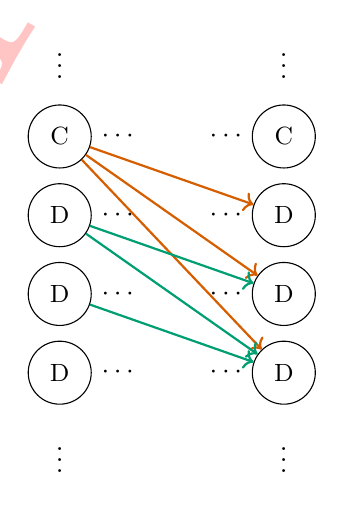
\begin{tikzpicture}[node distance=10mm, auto=center]
						\tikzstyle{main} = [circle, draw, minimum size=0.8cm, font=\small]
						\tikzstyle{source} = [circle, draw, minimum size=0.8cm, font=\small, fill=green!20]
						\tikzstyle{dest} = [circle, draw, minimum size=0.8cm, font=\small, fill=blue!20]

						% Left column (tree nodes)
						\node (dots_s_top) {\vdots};
						\node[main] (3s) [below of=dots_s_top] {C};
						\node[right=0cm of 3s] {$\cdots$};
						\node[main] (4s) [below of=3s] {D};
						\node[right=0cm of 4s] {$\cdots$};
						\node[main] (5s) [below of=4s] {D};
						\node[right=0cm of 5s] {$\cdots$};
						\node[main] (6s) [below of=5s] {D};
						\node[right=0cm of 6s] {$\cdots$};
						\node (dots_s_bottom) [below of=6s] {\vdots};

						% Right column (destinations)
						\node (dots_d_top) [right=2.5cm of dots_s_top] {\vdots};
						\node[main] (1d) [below of=dots_d_top] {C};
						\node[left=0cm of 1d] {$\cdots$};
						\node[main] (2d) [below of=1d] {D};
						\node[left=0cm of 2d] {$\cdots$};
						\node[main] (3d) [below of=2d] {D};
						\node[left=0cm of 3d] {$\cdots$};
						\node[main] (4d) [below of=3d] {D};
						\node[left=0cm of 4d] {$\cdots$};
						\node (dots_d_bottom) [below of=4d] {\vdots};

						% Arrows
						\draw[oiVermillion, ->, thick] (3s) -- (2d);
						\draw[oiVermillion, ->, thick] (3s) -- (4d);
						\draw[oiVermillion, ->, thick] (3s) -- (3d);

						\draw[oiGreen, ->, thick] (4s) -- (4d);
						\draw[oiGreen, ->, thick] (4s) -- (3d);

						\draw[oiGreen, ->, thick] (5s) -- (4d);
					\end{tikzpicture}
					\caption{}
					\label{fig:sub2}
				\end{subfigure}
				\hfill % Space between subfigures
				\tikzset{main/.style = {draw, circle, thick, minimum size=8mm, inner sep=0pt}}
				\begin{subfigure}[b]{0.3\textwidth}
					\centering
					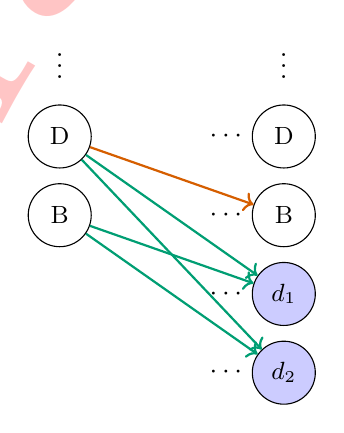
\begin{tikzpicture}[node distance=10mm, auto=center]
						\tikzstyle{main} = [circle, draw, minimum size=0.8cm, font=\small]
						\tikzstyle{source} = [circle, draw, minimum size=0.8cm, font=\small, fill=green!20]
						\tikzstyle{dest} = [circle, draw, minimum size=0.8cm, font=\small, fill=blue!20]

						% Left column (original destinations)
						\node (dots_s_top) {\vdots};
						\node[main] (7s) [below of=dots_s_top] {D};
						\node[main] (9s) [below of=7s] {B};

						% Right column (bipartite graph destinations)
						\node (dots_d_top) [right=2.5cm of dots_s_top] {\vdots};
						\node[main] (5d) [below of=dots_d_top] {D};
						\node[left=0cm of 5d] {$\cdots$};
						\node[main] (6d) [below of=5d] {B};
						\node[left=0cm of 6d] {$\cdots$};
						\node[dest] (8d) [below of=6d] {$d_1$};
						\node[left=0cm of 8d] {$\cdots$};
						\node[dest] (9d) [below of=8d] {$d_2$};
						\node[left=0cm of 9d] {$\cdots$};

						% Arrows
						\draw[oiVermillion, ->, thick] (7s) -- (6d);
						\draw[oiGreen, ->, thick] (7s) -- (8d);
						\draw[oiGreen, ->, thick] (7s) -- (9d);
						\draw[oiGreen, ->, thick] (9s) -- (8d);
						\draw[oiGreen, ->, thick] (9s) -- (9d);
					\end{tikzpicture}
					\caption{}
					\label{fig:sub3}
				\end{subfigure}
			\end{minipage}
		}% End scalebox
		\caption{Small Example for $\mathcal{O}(n^2)$ MWPBM Reduction. Green edges: 0, Red edges: 1.}
		\label{fig:reduction_small_examples}
	\end{figure}
\end{frame}

\begin{frame}{Example: $\mathcal{O}(np)$ MWPBM Reduction}
	\centering
	\begin{figure}[H]
		\centering
		\scalebox{0.9}{%
			\tikzset{main/.style = {draw, circle, thick, minimum size=8mm, inner sep=0pt}}
		\begin{subfigure}[b]{0.3\textwidth}
			\centering
			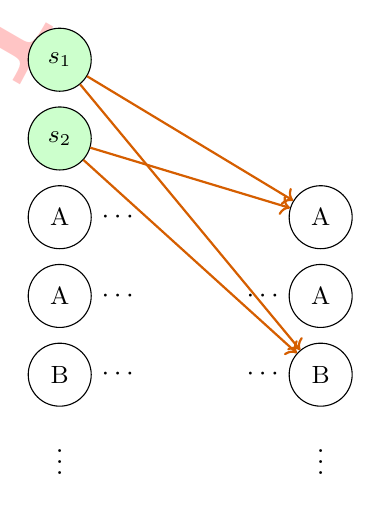
\begin{tikzpicture}[node distance=10mm, auto=center]
				\tikzstyle{main} = [circle, draw, minimum size=0.8cm, font=\small]
				\tikzstyle{source} = [circle, draw, minimum size=0.8cm, font=\small, fill=green!20]
				\tikzstyle{dest} = [circle, draw, minimum size=0.8cm, font=\small, fill=blue!20]

				% Left column (sources)
				\node[source] (1s) {$s_1$};
				\node[source] (2s) [below of=1s] {$s_2$};
				\node[main] (3s) [below of=2s] {A};
				\node[right=0cm of 3s] {$\cdots$};
				\node[main] (4s) [below of=3s] {A};
				\node[right=0cm of 4s] {$\cdots$};
				\node[main] (5s) [below of=4s] {B};
				\node[right=0cm of 5s] {$\cdots$};
				\node (dots_s) [below of=5s] {\vdots}; % Vertical dots

				% Right column (destinations)
				\node[main] (1d) [right=2.5cm of 3s] {A};
				\node[main] (2d) [below of=1d] {A};
				\node[left=0cm of 2d] {$\cdots$};
				\node[main] (3d) [below of=2d] {B};
				\node[left=0cm of 3d] {$\cdots$};
				\node (dots_d) [below of=3d] {\vdots}; % Vertical dots

				% Arrows
				\draw[oiVermillion, ->, thick] (1s) -- (1d);
				\draw[oiVermillion, ->, thick] (1s) -- (3d);
				\draw[oiVermillion, ->, thick] (2s) -- (1d);
				\draw[oiVermillion, ->, thick] (2s) -- (3d);
			\end{tikzpicture}
			\caption{}
			\label{fig:sub1}
		\end{subfigure}
		\hfill % Space between subfigures
		\tikzset{main/.style = {draw, circle, thick, minimum size=8mm, inner sep=0pt}}
		\begin{subfigure}[b]{0.3\textwidth}
			\centering
			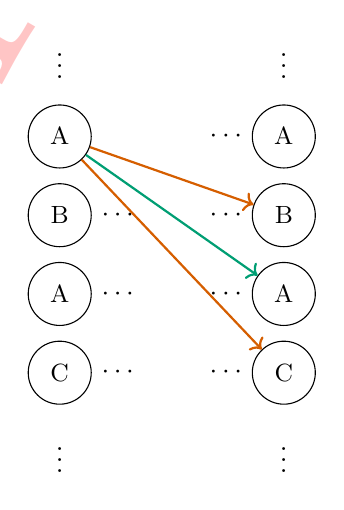
\begin{tikzpicture}[node distance=10mm, auto=center]
				\tikzstyle{main} = [circle, draw, minimum size=0.8cm, font=\small]
				\tikzstyle{source} = [circle, draw, minimum size=0.8cm, font=\small, fill=green!20]
				\tikzstyle{dest} = [circle, draw, minimum size=0.8cm, font=\small, fill=blue!20]

				% Left column (tree nodes)
				\node (dots_s_top) {\vdots};
				\node[main] (3s) [below of=dots_s_top] {A};
				\node[main] (4s) [below of=3s] {B};
				\node[right=0cm of 4s] {$\cdots$};
				\node[main] (5s) [below of=4s] {A};
				\node[right=0cm of 5s] {$\cdots$};
				\node[main] (6s) [below of=5s] {C};
				\node[right=0cm of 6s] {$\cdots$};
				\node (dots_s_bottom) [below of=6s] {\vdots};

				% Right column (destinations)
				\node (dots_d_top) [right=2.5cm of dots_s_top] {\vdots};
				\node[main] (1d) [below of=dots_d_top] {A};
				\node[left=0cm of 1d] {$\cdots$};
				\node[main] (2d) [below of=1d] {B};
				\node[left=0cm of 2d] {$\cdots$};
				\node[main] (3d) [below of=2d] {A};
				\node[left=0cm of 3d] {$\cdots$};
				\node[main] (4d) [below of=3d] {C};
				\node[left=0cm of 4d] {$\cdots$};
				\node (dots_d_bottom) [below of=4d] {\vdots};

				% Arrows
				\draw[oiVermillion, ->, thick] (3s) -- (2d);
				\draw[oiVermillion, ->, thick] (3s) -- (4d);
				\draw[oiGreen, ->, thick] (3s) -- (3d);
			\end{tikzpicture}
			\caption{}
			\label{fig:sub2}
		\end{subfigure}
		\hfill % Space between subfigures
		\tikzset{main/.style = {draw, circle, thick, minimum size=8mm, inner sep=0pt}}
		\begin{subfigure}[b]{0.3\textwidth}
			\centering
			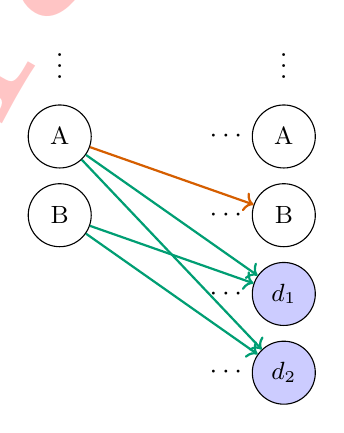
\begin{tikzpicture}[node distance=10mm, auto=center]
				\tikzstyle{main} = [circle, draw, minimum size=0.8cm, font=\small]
				\tikzstyle{source} = [circle, draw, minimum size=0.8cm, font=\small, fill=oiGreen!20]
				\tikzstyle{dest} = [circle, draw, minimum size=0.8cm, font=\small, fill=blue!20]

				% Left column (original destinations)
				\node (dots_s_top) {\vdots};
				\node[main] (7s) [below of=dots_s_top] {A};
				\node[main] (9s) [below of=7s] {B};

				% Right column (bipartite graph destinations)
				\node (dots_d_top) [right=2.5cm of dots_s_top] {\vdots};
				\node[main] (5d) [below of=dots_d_top] {A};
				\node[left=0cm of 5d] {$\cdots$};
				\node[main] (6d) [below of=5d] {B};
				\node[left=0cm of 6d] {$\cdots$};
				\node[dest] (8d) [below of=6d] {$d_1$};
				\node[left=0cm of 8d] {$\cdots$};
				\node[dest] (9d) [below of=8d] {$d_2$};
				\node[left=0cm of 9d] {$\cdots$};

				% Arrows
				\draw[oiVermillion, ->, thick] (7s) -- (6d);
				\draw[oiGreen, ->, thick] (7s) -- (8d);
				\draw[oiGreen, ->, thick] (7s) -- (9d);
				\draw[oiGreen, ->, thick] (9s) -- (8d);
				\draw[oiGreen, ->, thick] (9s) -- (9d);
			\end{tikzpicture}
			\caption{}
			\label{fig:sub3}
		\end{subfigure}
		}
		\caption{Small Example of $\mathcal{O}(np)$ MWPBM Reduction. Green edges: 0, Red edges: 1..}
	\end{figure}
\end{frame}

\begin{frame}{$p$--sortable Automata Index~[\cite{cotumaccio2021indexing}]}
	\begin{columns}[c]
		\column{0.55\textwidth}
		\begin{block}{\textcolor{white}{\textbf{Main Result}}}
			Let $\mathcal{A}$ be a \textcolor{oiBlue}{\textbf{$p$--sortable automaton}}. There exists a \textcolor{oiGreen}{\textbf{compressed data structure}} for $\mathcal{A}$ that supports \textcolor{oiPurple}{\textbf{subpath queries}} on a query word $\alpha$ of length $m$ in
			\[\mathbf{O(mp^2\log\log(p|\Sigma|))}\text{ time}\]
		\end{block}

		\column{0.45\textwidth}
		\textcolor{oiGreen}{\textbf{Space Complexity}}
		\begin{block}{\textcolor{white}{\textbf{DFA Case}}}
			$\mathbf{\log(|\Sigma|) + \log p + 2}$ bits per edge
		\end{block}

		\vspace{0.2cm}
		\begin{block}{\textcolor{white}{\textbf{NFA Case}}}
			$\mathbf{\log(|\Sigma|) + 2\log p + 2}$ bits per edge
		\end{block}
	\end{columns}
	\vspace{0.3cm}
	\textcolor{oiRed}{\textbf{Key Properties}}
	\begin{itemize}
		\item \textbf{Efficiency:} Efficient subpath query time
		\item \textbf{Generality:} Works for both DFA and NFA
		\item \textbf{Scalability:} Performance and space depend on $p$
	\end{itemize}
\end{frame}

\end{document}

